\documentclass[t,8pt]{beamer}

%%% packages
\geometry{paperwidth=140mm,paperheight=105mm}
\usefonttheme[onlymath]{serif}

\usepackage{kotex,amsmath,tabto}

\usepackage{tabularx}
%X is not not centered, text moded
\newcolumntype{Y}{>{\centering\arraybackslash}X} % centered, text-moded
\newcolumntype{M}{>{$}X<{$}} % math-moded
\newcolumntype{N}{>{$}Y<{$}} %centered and math-moded

\usepackage{gensymb} %\degree

%%% counters, commands, environments
\newcounter{num}
\resetcounteronoverlays{num}

\newenvironment{defi}[1]{\refstepcounter{num}\begin{block}{정의 \arabic{num}#1}}{\end{block}}
\newenvironment{theo}[1]{\refstepcounter{num}\begin{block}{정리 \arabic{num}#1}}{\end{block}}
\newenvironment{prob}[1]{\refstepcounter{num}\begin{block}{문제 \arabic{num}#1}}{\end{block}}
\newenvironment{exam}[1]{\refstepcounter{num}\begin{block}{예시 \arabic{num}#1}}{\end{block}}

\newcommand{\pb}[1]%\Phantom + fBox
{\fbox{\phantom{\ensuremath{#1}}}}
\renewcommand{\arraystretch}{1.5}
\newcommand{\red}[1]{\color{red}{#1}}
\newcommand{\ivs}{\centering\strut\vspace*{-\baselineskip}\newline}%image vertical setting

%%% title
\title{삼각함수}
\institute[ibedu]{아이비에듀}
\date{\today}

%%% toc
\AtBeginSection[]
{\begin{frame}
    \frametitle{목차}
    \tableofcontents[currentsection]
  \end{frame}}


\begin{document}

%%
\frame{\titlepage}

%%%%
\section{삼각함수의 뜻}

%%%
\subsection{호도법}
%%
\begin{frame}[t]{\subsecname}
%
\begin{prob}{}
`인치(inch)'는  미국에서 주로 사용되는 길이 단위로 \(1\;\text{inch}\)는 약 \(2.54\;\text{cm}\)에 해당한다.

(1) \(3\;\text{inch}=\fbox{\uncover<2->{\red{7.62}}}\;\text{cm}\)
\tabto{.5\textwidth}
(2) \(0.5\;\text{inch}=\fbox{\uncover<2->{\red{1.27}}}\;\text{cm}\)
\end{prob}

\pause\pause\bigskip
지금까지 각도의 크기를 나타내는 단위는 도(\degree)였다.
각도를 나타내는 새로운 단위로 라디안(rad)이 있다.
이때, \(180\degree = \pi\;\text{rad}\)이다.

\pause
%
\begin{exam}{}
\begin{enumerate}
\item
위의 식의 양변에 2를 곱하면 \(360\degree=2\pi\;\text{rad}\)이다.
\item
마찬가지로, 양변을 3으로 나누면 \(60\degree=\frac\pi3\;\text{rad}\)이다.
\end{enumerate}
\end{exam}

%
\pause
\begin{prob}{) 다음 빈칸을 채워 넣어라.}
\begin{tabularx}{\textwidth}{|N|N|N|N|N|N|N|N|N|N|N|}
\hline
 0\degree
&30\degree
&45\degree
&60\degree
&\uncover<6->{\color{red}90\degree}
&\uncover<6->{\color{red}120\degree}
&\uncover<6->{\color{red}135\degree}
&150\degree
&180\degree
&270\degree
&360\degree
\\\hline
0
&\uncover<6->{\color{red}\frac\pi6}
&\uncover<6->{\color{red}\frac\pi4}
&\frac\pi3
&\frac\pi2
&\frac23\pi
&\frac34\pi
&\uncover<6->{\color{red}\frac56\pi}
&\pi
&\uncover<6->{\color{red}\frac32\pi}
&2\pi
\\\hline
\end{tabularx}
\end{prob}

\pause\pause\bigskip
%
\begin{prob}{) 정사각형과 정삼각형의 한 내각의 크기를 라디안으로 구하여라.}
\begin{center}
\includegraphics<7>[width=.3\textwidth]{img/1-1_radian_1}
\includegraphics<8>[width=.3\textwidth]{img/1-1_radian_2}
\end{center}
\end{prob}
\end{frame}

%%%
\subsection{부채꼴의 호의 길이와 넓이}

%%
\begin{frame}{\subsecname}
\begin{minipage}{.6\textwidth}
%
\begin{prob}{}
오른쪽 그림과 같이 반지름의 길이가 \(10\)이고 중심각의 크기가 \(45\)\degree인 부채꼴의 호의 길이 \(l\)과 넓이 \(S\)를 각각 구하여라.
\end{prob}
\end{minipage}
\begin{minipage}{.3\textwidth}
\centering
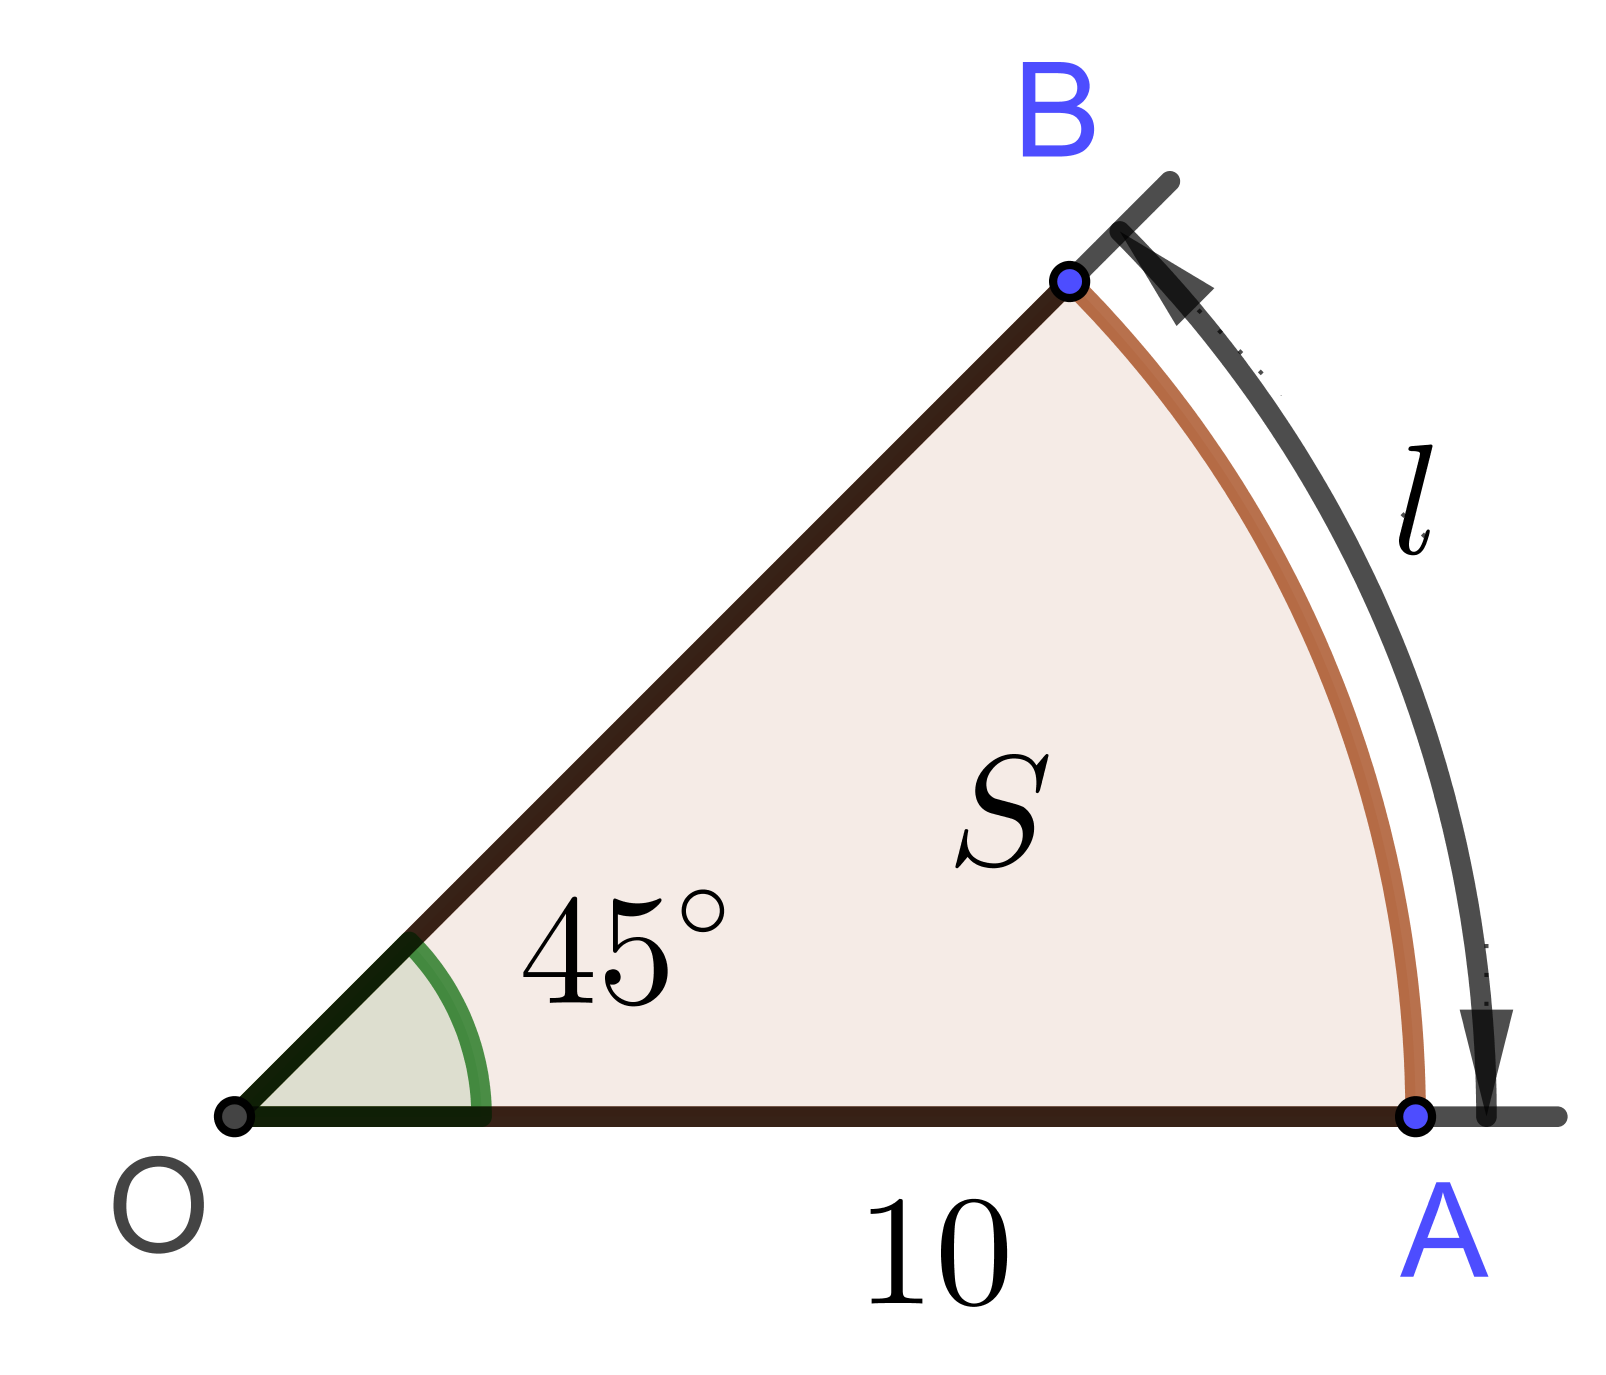
\includegraphics[width=.7\textwidth]{img/1-2_arc_1}
\end{minipage}
\uncover<2>{
\begin{align*}
l&=2\times\pi\times10\times\frac{45\degree}{360\degree}=\frac52\pi.\\
S&=\pi\times10^2\times\frac{45\degree}{360\degree}=\frac{25}2\pi
\end{align*}
}

\pause\pause\vspace{-50pt}
\begin{minipage}{.6\textwidth}
%
\begin{theo}{) 부채꼴의 호의 길이와 넓이}
반지름의 길이가 \(r\)이고 중심각의 크기가 \(\theta\)인 부채꼴의 호의 길이 \(l\)과 넓이 \(S\)이면,\\
\begin{itemize}
\item
\(l=r\theta\)
\item
\(S=\frac12r^2\theta\uncover<5->{=\frac12rl.}\)
\end{itemize}
\end{theo}
\end{minipage}
\begin{minipage}{.3\textwidth}
\centering
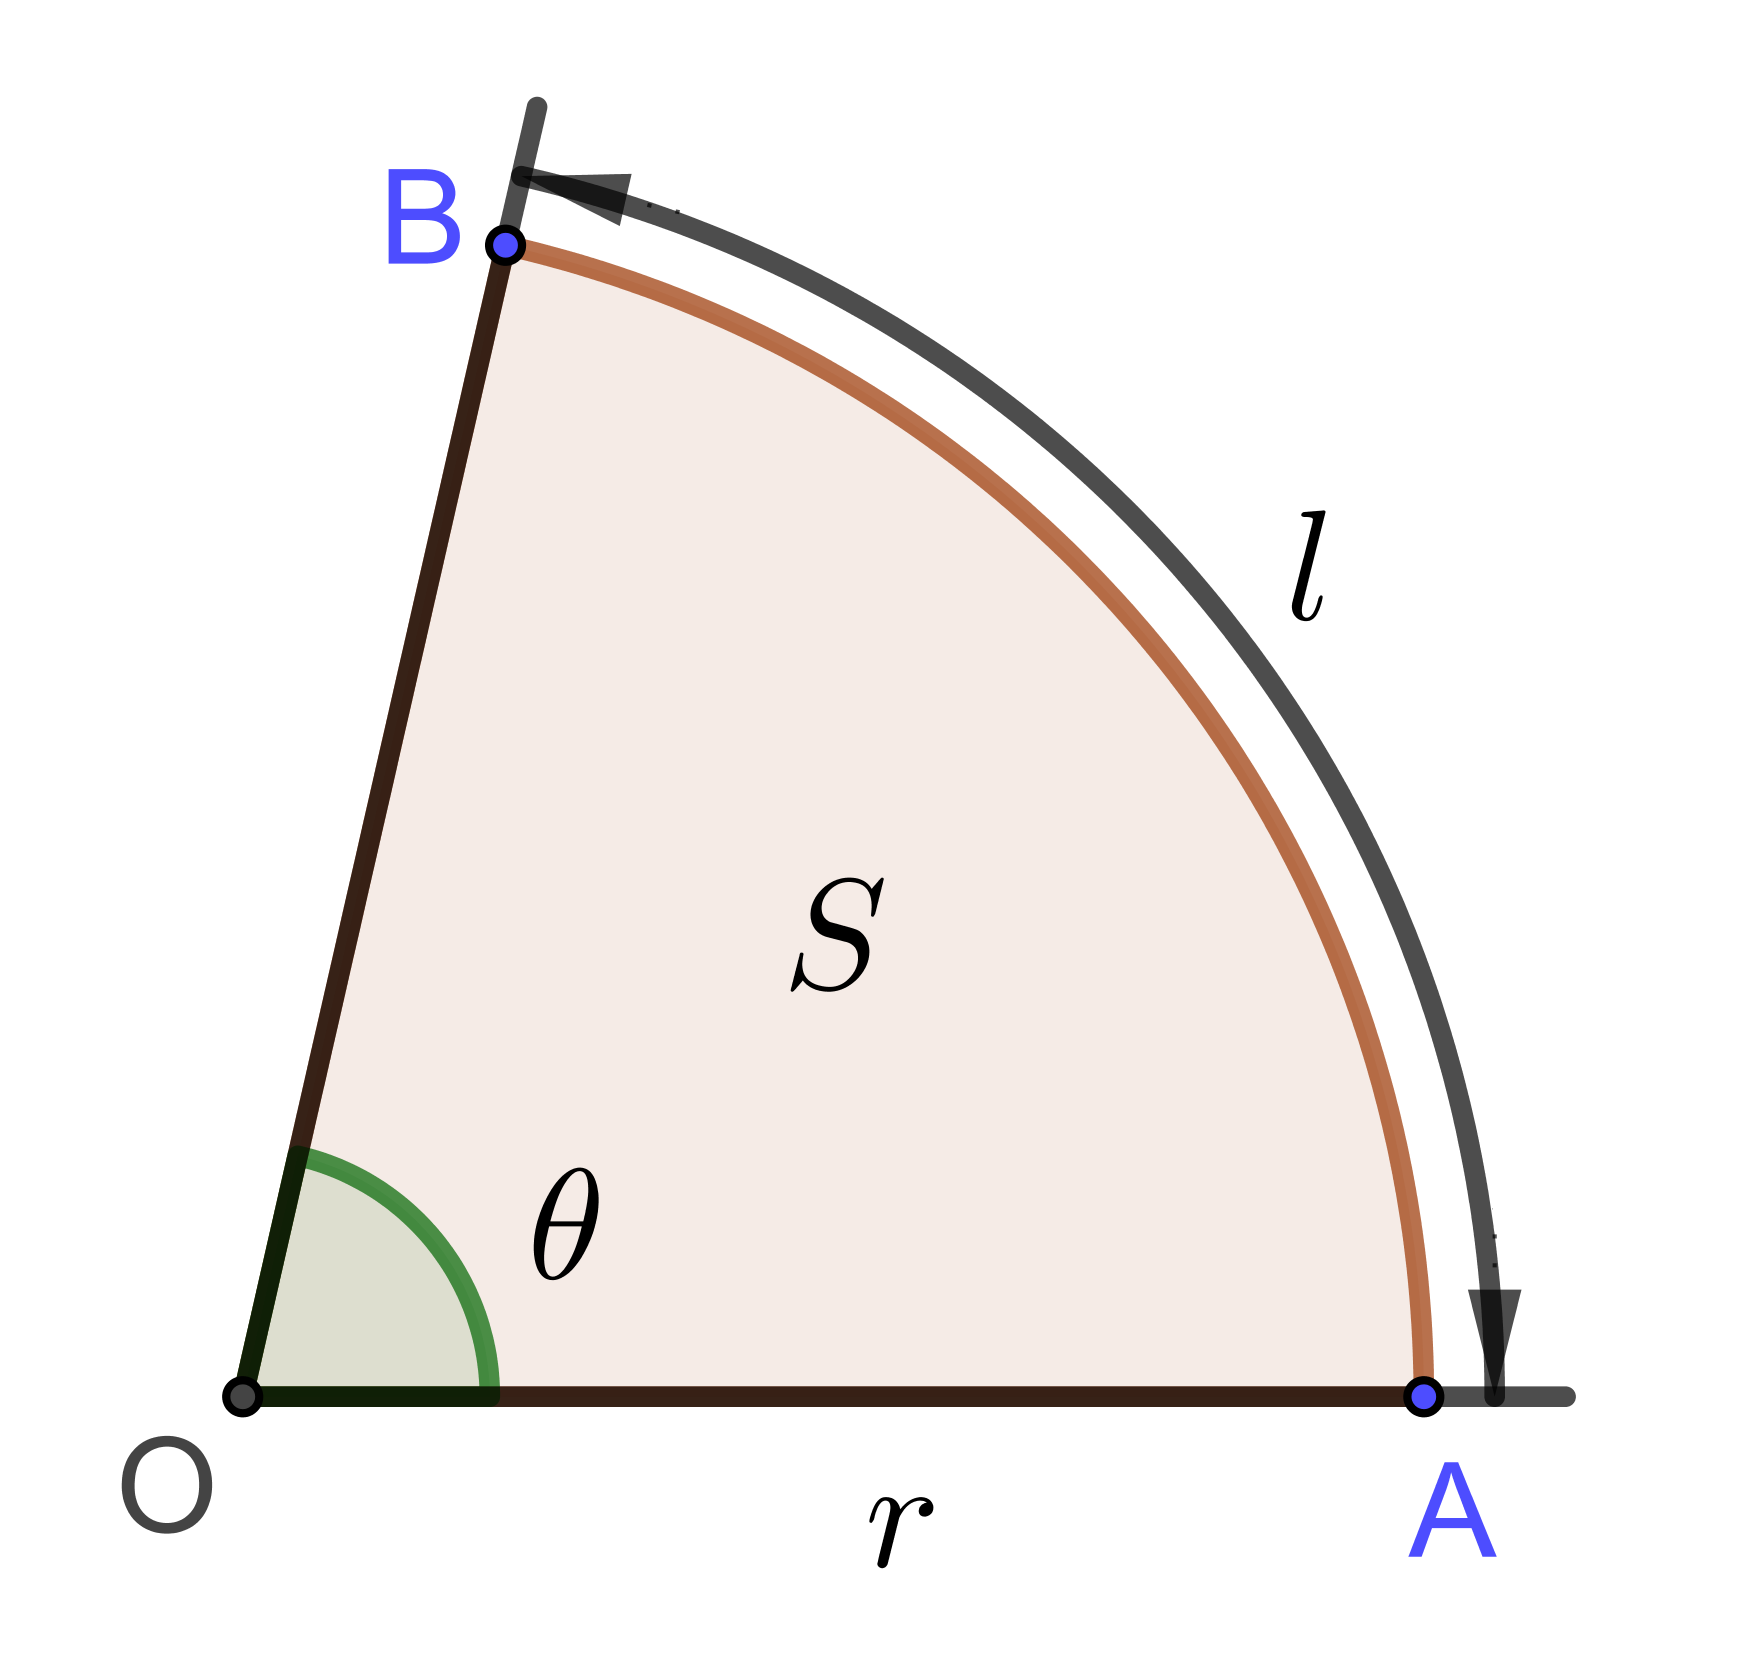
\includegraphics[width=.7\textwidth]{img/1-2_arc_2}
\end{minipage}

\bigskip
\pause\pause
\begin{minipage}{.6\textwidth}
%
\begin{prob}{}
\begin{align*}
l=&\uncover<6->{4\times\frac34\pi=\color{red}{3\pi}}\\
S=&\uncover<6->{\frac12\times4^2\times\frac34\pi=\color{red}{6\pi}}
\end{align*}
\end{prob}
\end{minipage}
\begin{minipage}{.3\textwidth}
\centering
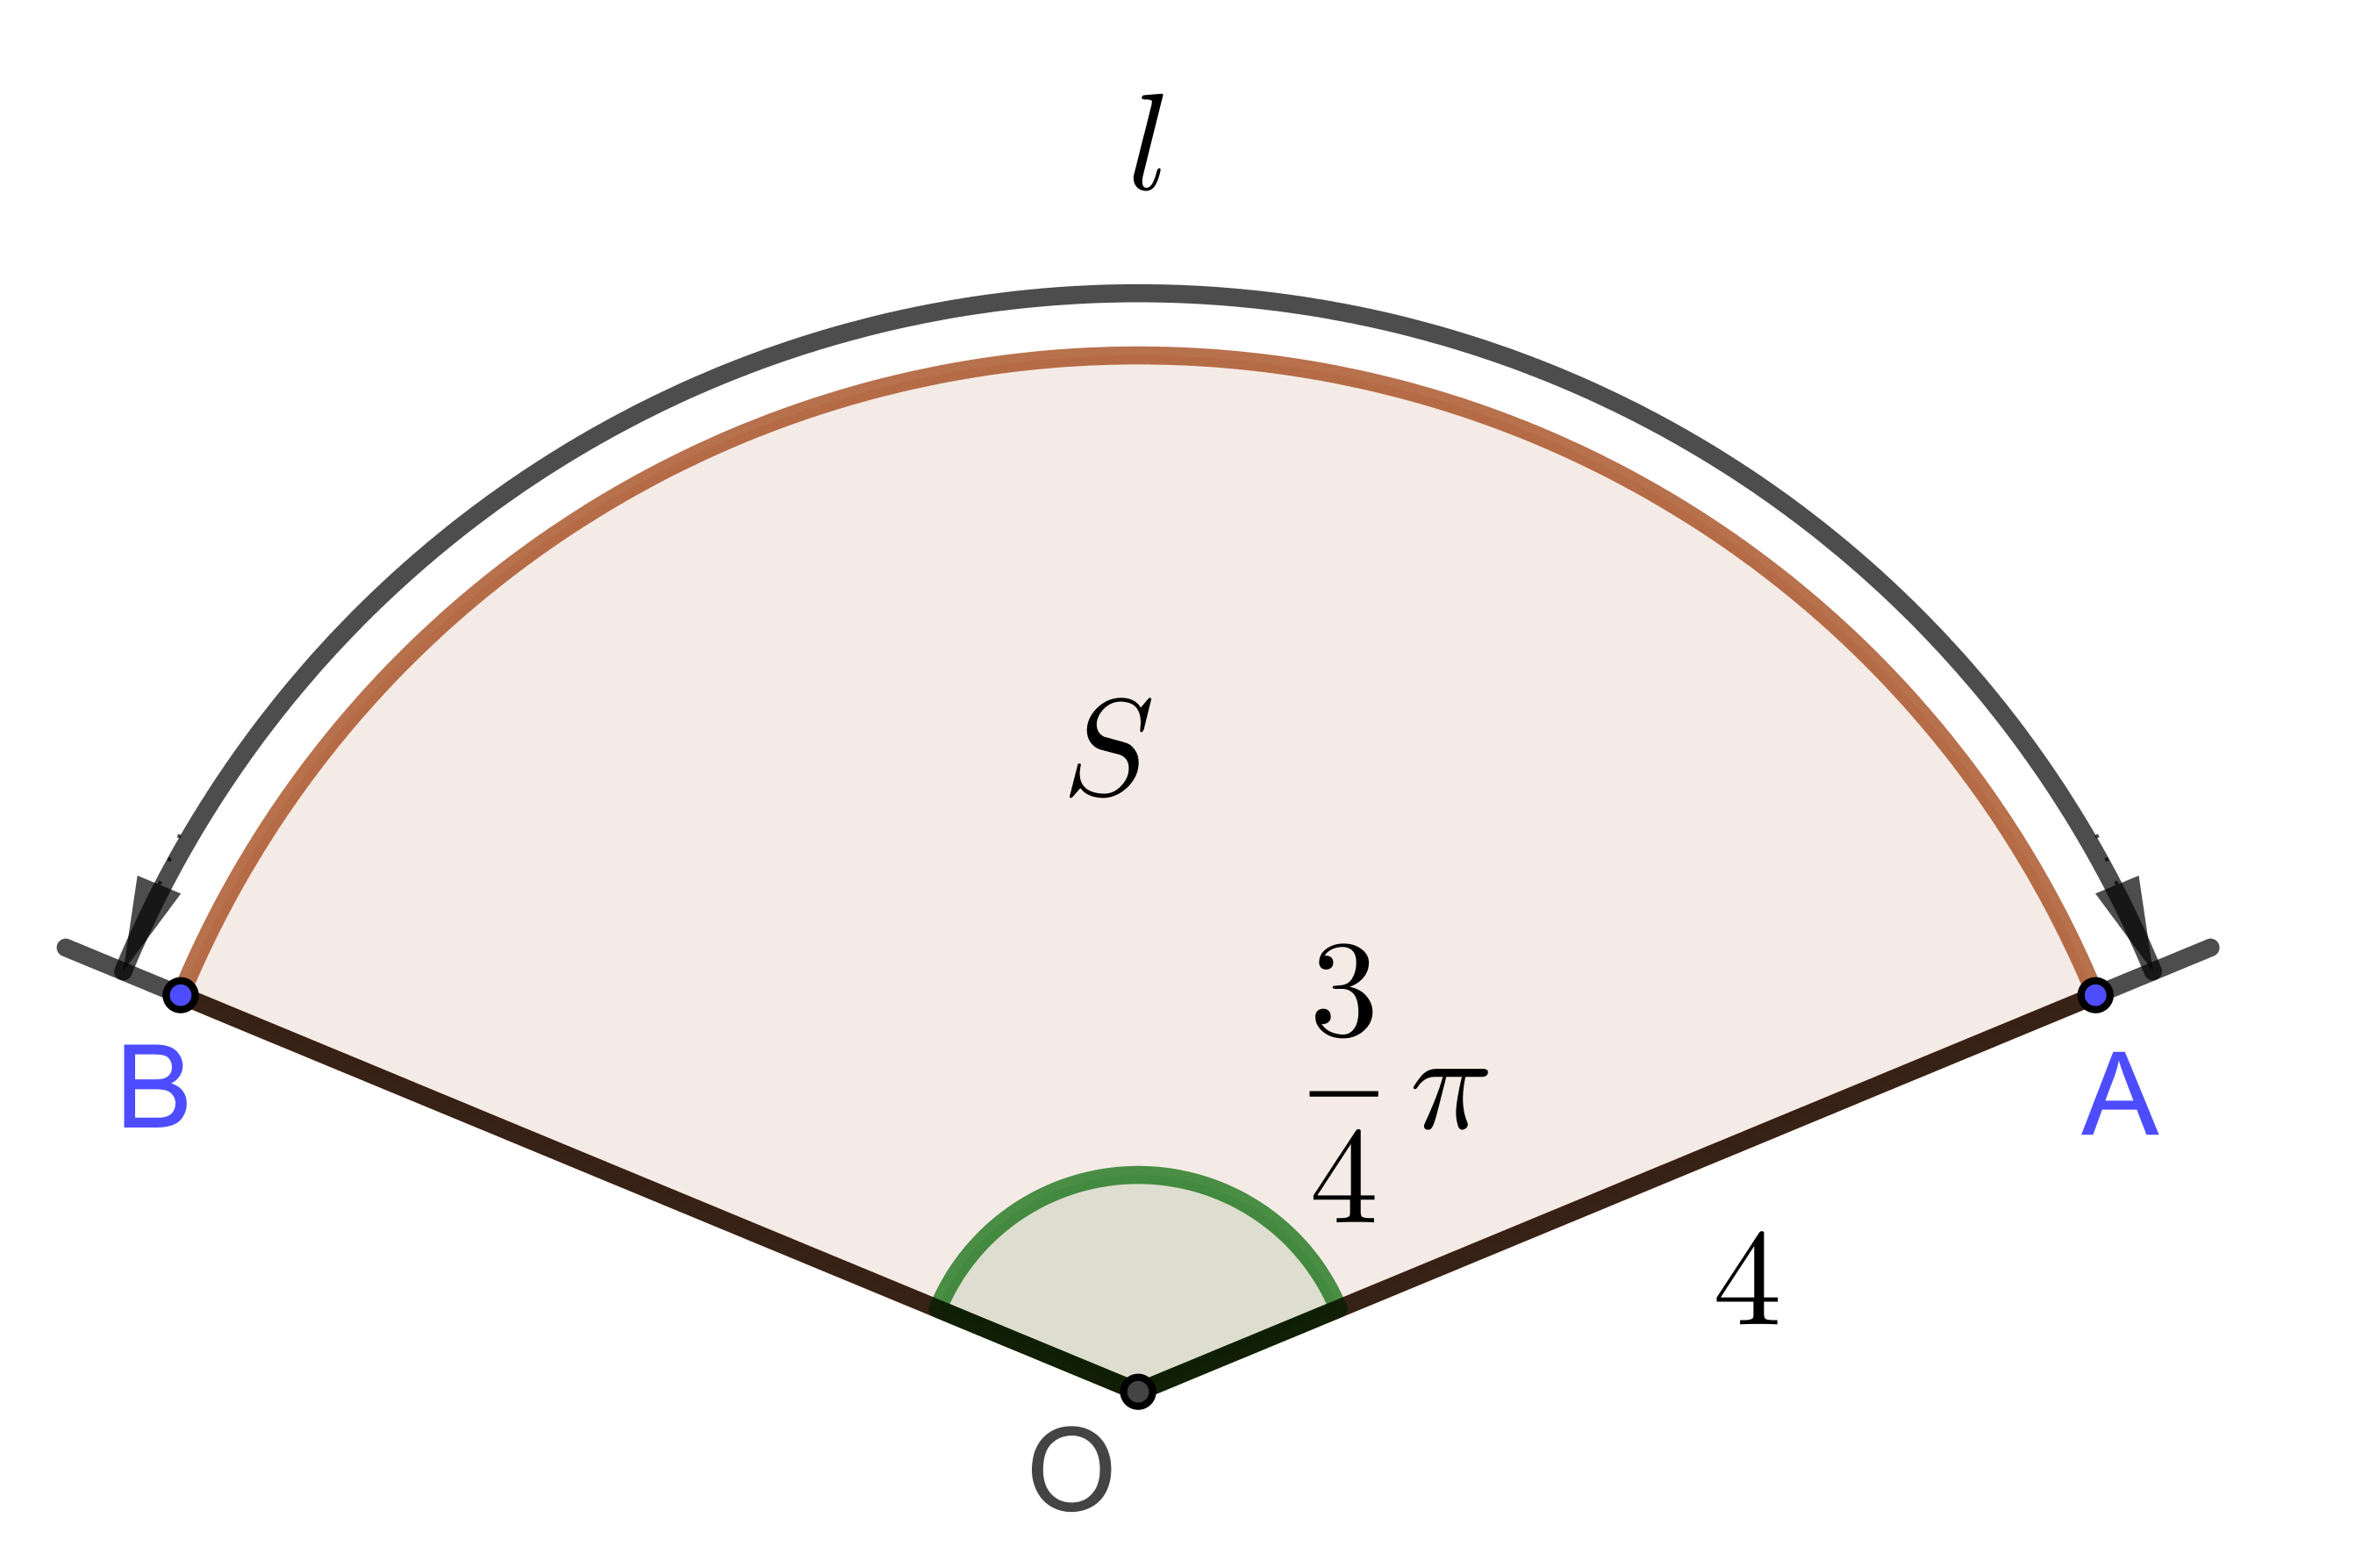
\includegraphics[width=\textwidth]{img/1-2_arc_3}
\end{minipage}
\end{frame}

%%%
\subsection{삼각비(복습)}

%%
\begin{frame}{\subsecname}
\begin{minipage}{.6\textwidth}
%
\begin{defi}{) 삼각비}
\[\sin A=\frac ac,\quad\cos A=\frac bc,\quad\tan A=\frac ab\]
\end{defi}
\end{minipage}
\begin{minipage}{.3\textwidth}
\centering
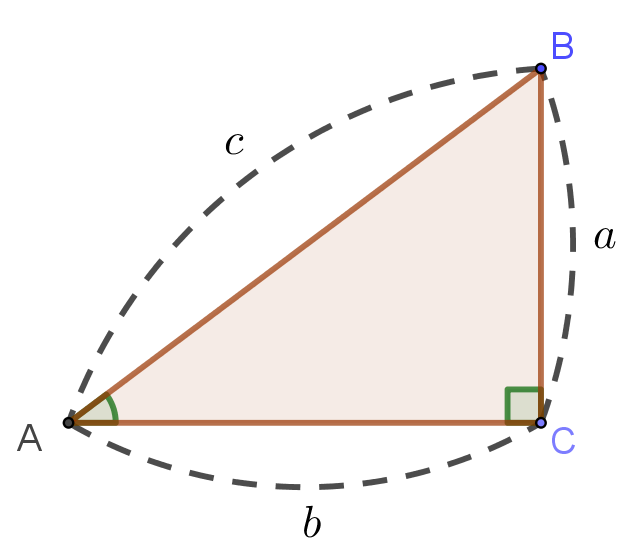
\includegraphics[width=.7\textwidth]{img/1-3_tratio_1}
\end{minipage}

\pause
\begin{minipage}[t]{.6\textwidth}
%
\begin{prob}{) \(\frac\pi3\)의 삼각비를 구하여라.}
\[\sin\frac\pi3=\uncover<3->{\frac{\sqrt3}2,}\quad\cos\frac\pi3=\uncover<3->{\frac12,}\quad\tan\frac\pi3=\uncover<3->{\sqrt3}\]
\end{prob}
\end{minipage}
\begin{minipage}[t]{.3\textwidth}
\ivs
\includegraphics<3->[width=.6\textwidth]{img/1-3_tratio_2}
\end{minipage}

%
\pause\pause
\begin{prob}{) 다음 값들을 계산하여라.}
\medskip
(1) \(\sin\frac\pi6=\uncover<5->{\frac12}\)
\tabto{.3\textwidth}\(\cos\frac\pi6=\uncover<5->{\frac{\sqrt3}2}\)
\tabto{.6\textwidth}\(\tan\frac\pi6=\uncover<5->{\frac{\sqrt3}3}\)\\[10pt]
(2) \(\sin\frac\pi4=\uncover<5->{\frac{\sqrt2}2}\)
\tabto{.3\textwidth}\(\cos\frac\pi4=\uncover<5->{\frac{\sqrt2}2}\)
\tabto{.6\textwidth}\(\tan\frac\pi4=\uncover<5->{1}\)\\[10pt]\pause\pause
(3) \(\left(\sin\frac\pi6\right)^2+\left(\cos\frac\pi6\right)^2=\uncover<7->1\)\\[10pt]
(4) \(\left(\sin\frac\pi4\right)^2+\left(\cos\frac\pi4\right)^2=\uncover<7->1\)
\end{prob}
\end{frame}

%%%
\subsection{삼각함수}

%%
\begin{frame}{\subsecname}
\begin{minipage}{.7\textwidth}
%
\begin{defi}{) 삼각함수}
\(x\)축 위의 점 \(A=(r,0)\)을 원점을 중심으로 시계반대방향으로 \(\theta\)만큼 회전 시킨 점을 \(P(x,y)\)라고 하면,
%양수 \(r\)에 대하여 점 \(A=(r,0)\)을 원 \(x^2+y^2=r^2\)을 따라 시계 반대 방향\footnotemark으로 \(\theta\)만큼 회전시킨 점을 \(P(x,y)\)라고 할 때,
\[\sin\theta=\frac yr,\quad\cos\theta=\frac xr,\quad\tan\theta=\frac yx\]
\end{defi}
\end{minipage}
\begin{minipage}{.25\textwidth}
\centering
\vspace{20pt}
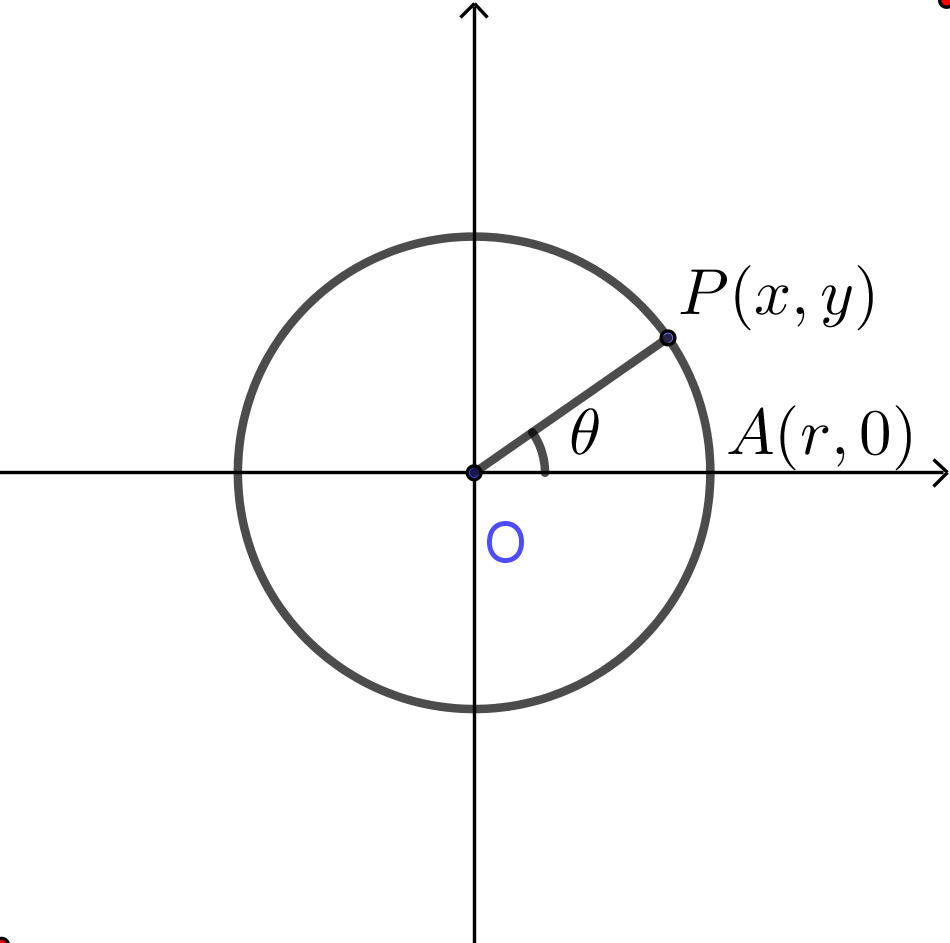
\includegraphics[width=.9\textwidth]{img/1-4_tfunction_1}
\end{minipage}
이다.
이때, \(\overrightarrow{OA}\)를 시초선, \(\overrightarrow{OP}\)를 동경이라고 부른다(\(r>0\)).

\pause\bigskip
%
\begin{prob}{) 다음 삼각함수의 값들을 계산하여라.}
\begin{minipage}[t]{.24\textwidth}\footnotesize
\begin{align*}
(1) 	&\sin\frac\pi6=\uncover<3->{\frac12}\\
	&\cos\frac\pi6=\uncover<3->{\frac{\sqrt3}2}\\
	&\tan\frac\pi6=\uncover<3->{\frac1{\sqrt3}=\frac{\sqrt3}3}
\end{align*}
\end{minipage}
\begin{minipage}[t]{.24\textwidth}
\ivs
\includegraphics<2>[width=\textwidth]{img/1-4_tfunction_2}
\includegraphics<3->[width=\textwidth]{img/1-4_tfunction_2-1}
\end{minipage}
\begin{minipage}[t]{.24\textwidth}\footnotesize
\begin{align*}
(2) 	&\sin\frac\pi4=\uncover<3->{\frac1{\sqrt2}=\frac{\sqrt2}2}\\
	&\cos\frac\pi4=\uncover<3->{\frac1{\sqrt2}=\frac{\sqrt2}2}\\
	&\tan\frac\pi4=\uncover<3->{\frac11=1}
\end{align*}
\end{minipage}
\begin{minipage}[t]{.24\textwidth}
\ivs
\includegraphics<2>[width=\textwidth]{img/1-4_tfunction_2}
\includegraphics<3->[width=\textwidth]{img/1-4_tfunction_2-2}
\end{minipage}
\end{prob}
\end{frame}

%%
\begin{frame}{\subsecname}
\begin{minipage}[t]{.24\textwidth}\footnotesize
\begin{align*}
(3) 	&\sin\frac\pi3=\uncover<2->{\frac{\sqrt3}2}\\
	&\cos\frac\pi3=\uncover<2->{\frac12}\\
	&\tan\frac\pi3=\uncover<2->{\sqrt3}
\end{align*}
\end{minipage}
\begin{minipage}[t]{.24\textwidth}
\ivs
\includegraphics<1>[width=\textwidth]{img/1-4_tfunction_2}
\includegraphics<2->[width=\textwidth]{img/1-4_tfunction_2-3}
\end{minipage}
\begin{minipage}[t]{.24\textwidth}\footnotesize
\begin{align*}
(4) 	&\sin\frac\pi2=\uncover<2->{\frac11=1}\\
	&\cos\frac\pi2=\uncover<2->{\frac01=0}\\
	&\tan\frac\pi2=\uncover<2->{\frac10\:(\text{존재x})}
\end{align*}
\end{minipage}
\begin{minipage}[t]{.24\textwidth}
\ivs
\includegraphics<1>[width=\textwidth]{img/1-4_tfunction_2}
\includegraphics<2->[width=\textwidth]{img/1-4_tfunction_2-4}
\end{minipage}
\par\medskip
\begin{minipage}[t]{.24\textwidth}\footnotesize
\begin{align*}
(5) 	&\sin\frac23\pi=\uncover<2->{\frac{\sqrt3}2}\\
	&\cos\frac23\pi=\uncover<2->{\frac{-1}2=-\frac12}\\
	&\tan\frac23\pi=\uncover<2->{\frac{\sqrt3}{-1}=-\sqrt3}
\end{align*}
\end{minipage}
\begin{minipage}[t]{.24\textwidth}
\ivs
\includegraphics<1>[width=\textwidth]{img/1-4_tfunction_2}
\includegraphics<2->[width=\textwidth]{img/1-4_tfunction_2-5}
\end{minipage}
\begin{minipage}[t]{.24\textwidth}\footnotesize
\begin{align*}
(6) 	&\sin\frac34\pi=\uncover<2->{\frac1{\sqrt2}=\frac{\sqrt2}2}\\
	&\cos\frac34\pi=\uncover<2->{\frac{-1}{\sqrt2}=-\frac{\sqrt2}2}\\
	&\tan\frac34\pi=\uncover<2->{\frac{1}{-1}=-1}
\end{align*}
\end{minipage}
\begin{minipage}[t]{.24\textwidth}
\ivs
\includegraphics<1>[width=\textwidth]{img/1-4_tfunction_2}
\includegraphics<2->[width=\textwidth]{img/1-4_tfunction_2-6}
\end{minipage}
\par\medskip
\begin{minipage}[t]{.24\textwidth}\footnotesize
\begin{align*}
(7) 	&\sin\pi=\uncover<2->{\frac01=0}\\
	&\cos\pi=\uncover<2->{\frac{-1}1=-1}\\
	&\tan\pi=\uncover<2->{\frac0{-1}=0}
\end{align*}
\end{minipage}
\begin{minipage}[t]{.24\textwidth}
\ivs
\includegraphics<1>[width=\textwidth]{img/1-4_tfunction_2}
\includegraphics<2->[width=\textwidth]{img/1-4_tfunction_2-7}
\end{minipage}
\begin{minipage}[t]{.24\textwidth}\footnotesize
\begin{align*}
(8) 	&\sin\frac32\pi=\uncover<2->{\frac{-1}1=-1}\\
	&\cos\frac32\pi=\uncover<2->{\frac01=0}\\
	&\tan\frac32\pi=\uncover<2->{\frac{-1}0\:(\text{존재x})}
\end{align*}
\end{minipage}
\begin{minipage}[t]{.24\textwidth}
\ivs
\includegraphics<1>[width=\textwidth]{img/1-4_tfunction_2}
\includegraphics<2->[width=\textwidth]{img/1-4_tfunction_2-8}
\end{minipage}
\end{frame}

%%
\begin{frame}{\subsecname}
\begin{minipage}[t]{.26\textwidth}\footnotesize
\begin{align*}
(9) 	&\sin\frac53\pi=\uncover<2->{\frac{-\sqrt3}2=-\frac{\sqrt3}2}\\
	&\cos\frac53\pi=\uncover<2->{\frac12}\\
	&\tan\frac53\pi=\uncover<2->{\frac{-\sqrt3}1=-\sqrt3}
\end{align*}
\end{minipage}
\begin{minipage}[t]{.19\textwidth}
\ivs
\includegraphics<1>[width=\textwidth]{img/1-4_tfunction_2}
\includegraphics<2->[width=\textwidth]{img/1-4_tfunction_2-9}
\end{minipage}
\begin{minipage}[t]{.33\textwidth}\footnotesize
\begin{align*}
(10) 	&\sin\left(-\frac\pi3\right)=\uncover<2->{\frac{-\sqrt3}2=-\frac{\sqrt3}2}\\
	&\cos\left(-\frac\pi3\right)=\uncover<2->{\frac12}\\
	&\tan\left(-\frac\pi3\right)=\uncover<2->{\frac{-\sqrt3}1=-\sqrt3}
\end{align*}
\end{minipage}
\begin{minipage}[t]{.19\textwidth}
\ivs
\includegraphics<1>[width=\textwidth]{img/1-4_tfunction_2}
\includegraphics<2->[width=\textwidth]{img/1-4_tfunction_2-10}
\end{minipage}
\par\medskip
\begin{minipage}[t]{.26\textwidth}\footnotesize
\begin{align*}
(11) 	&\sin\frac{13}6\pi=\uncover<2->{\frac12}\\
	&\cos\frac{13}6\pi=\uncover<2->{\frac{\sqrt3}2}\\
	&\tan\frac{13}6\pi=\uncover<2->{\frac1{\sqrt3}=\frac{\sqrt3}3}
\end{align*}
\end{minipage}
\begin{minipage}[t]{.19\textwidth}
\ivs
\includegraphics<1>[width=\textwidth]{img/1-4_tfunction_2}
\includegraphics<2->[width=\textwidth]{img/1-4_tfunction_3-1}
\end{minipage}
\begin{minipage}[t]{.33\textwidth}\footnotesize
\begin{align*}
(12) 	&\sin\frac83\pi=\uncover<2->{\frac{\sqrt3}2}\\
	&\cos\frac83\pi=\uncover<2->{\frac{-1}2=-\frac12}\\
	&\tan\frac83\pi=\uncover<2->{\frac{\sqrt3}{-1}=-\sqrt3}
\end{align*}
\end{minipage}
\begin{minipage}[t]{.19\textwidth}
\ivs
\includegraphics<1>[width=\textwidth]{img/1-4_tfunction_2}
\includegraphics<2->[width=\textwidth]{img/1-4_tfunction_3-2}
\end{minipage}
\end{frame}

%%%
\subsection{삼각함수의 성질}

%%
\begin{frame}{\subsecname}
\begin{minipage}{.6\textwidth}
%
\begin{theo}{) 삼각함수의 성질}
\par\medskip
\begin{enumerate}[(1)]
\item
\(-1\le\sin\theta\le1\), \(-1\le\cos\theta\le1\)
\item
\(\sin^2\theta+\cos^2\theta=1\)
\item
\(\tan\theta=\frac{\sin\theta}{\cos\theta}\)
\end{enumerate}
\end{theo}
\end{minipage}
\begin{minipage}{.35\textwidth}
\centering
\vspace{20pt}
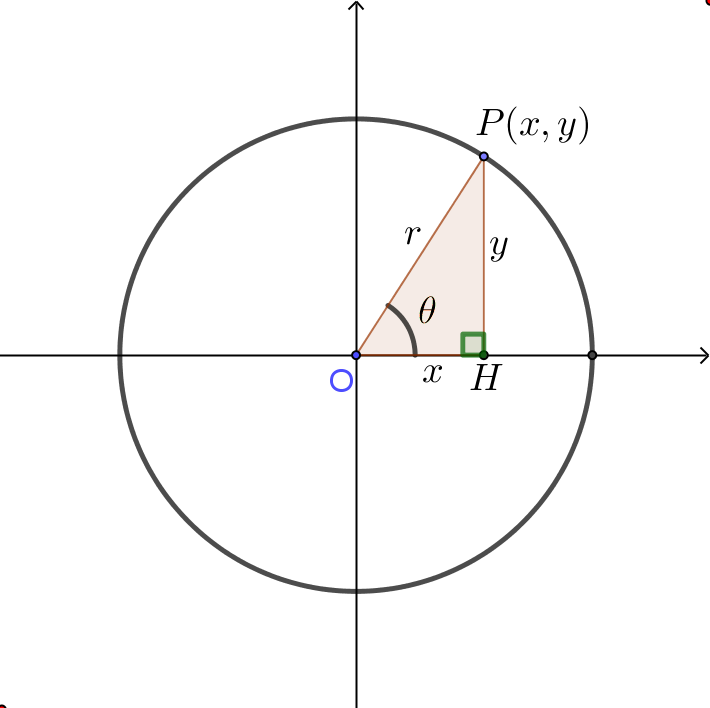
\includegraphics[width=.9\textwidth]{img/1-5_tproperty_1}
\end{minipage}

\begin{minipage}{.8\textwidth}
%
\begin{prob}{}
\par\medskip
\begin{enumerate}[(1)]
\item
\(2\sin^2\theta+3\sin\theta-2=0\)일 때, \(\sin\theta\)의 값을 구하시오.
\item
\(\sin\theta=\frac{2\sqrt2}3\)일 때, \(\cos\theta\)의 값으로 가능한 것을 모두 구하시오.
\item
\(\sin\theta=\frac35\), \(\cos\theta=\frac45\)일 때, \(\tan\theta\)의 값을 구하시오.
\item
\(\sin\theta=\frac{\sqrt{21}}5\)이고, \(0\le\theta\le\frac\pi2\)일 때, \(\tan\theta\)의 값을 구하여라.
\end{enumerate}
\end{prob}
\end{minipage}
\pause
\begin{minipage}{.15\textwidth}
\vspace{15pt}
\begin{enumerate}[(1)]
\item
\textcolor{red}{\(\frac12\)}
\item
\textcolor{red}{\(\pm\frac13\)}
\item
\textcolor{red}{\(\frac34\)}
\item
\textcolor{red}{\(\frac25\)}
\end{enumerate}
\end{minipage}
\end{frame}

%%%%
\section{삼각함수의 그래프}
%%%
\subsection{기본 그래프}

%%
\begin{frame}{\subsecname}
\setlength{\tabcolsep}{0pt}
%
\begin{prob}{) 다음 표를 완성하여라.}
\begin{tabularx}{\textwidth}{|@{\quad}N@{\quad\;\;}|N|N|N|N|N|N|N|N|N|N|N|N|N|}
\hline
\theta
&0
&\frac\pi6
&\frac\pi3
&\frac\pi2
&\frac23\pi
&\frac56\pi
&\pi
&\frac76\pi
&\frac43\pi
&\frac32\pi
&\frac53\pi
&\frac{11}6\pi
&2\pi
\\\hline
\sin\theta
&\uncover<2>{\red{0}}
&\frac12
&\uncover<2>{\red{\frac{\sqrt3}2}}
&\uncover<2>{\red{1}}
&\uncover<2>{\red{\frac{\sqrt3}2}}
&\uncover<2>{\red{\frac12}}
&\uncover<2>{\red{0}}
&\uncover<2>{\red{-\frac12}}
&\uncover<2>{\red{-\frac{\sqrt3}2}}
&\uncover<2>{\red{-1}}
&\uncover<2>{\red{-\frac{\sqrt3}2}}
&\uncover<2>{\red{-\frac12}}
&\uncover<2>{\red{0}}
\\\hline
\end{tabularx}
\end{prob}
%
\begin{prob}{) \(y=\sin x\)의 그래프를 그려라.}
\begin{minipage}{.7\textwidth}
\includegraphics<1>[width=\textwidth]{img/2-1_graph__grid}
\includegraphics<2>[width=\textwidth]{img/2-1_graph_1}
\end{minipage}
\begin{minipage}{.29\textwidth}
\uncover<2>{\small
\begin{itemize}
\item
\(-1\le\sin x\le 1\)
\item
\(\text{주기}=2\pi\)
\item
원점 대칭 (기함수)
\end{itemize}}
\end{minipage}
\end{prob}
\end{frame}

%%
\begin{frame}{\subsecname}
\setlength{\tabcolsep}{0pt}
%
\begin{prob}{) 다음 표를 완성하여라.}
\begin{tabularx}{\textwidth}{|@{\quad}N@{\quad\;\;}|N|N|N|N|N|N|N|N|N|N|N|N|N|}
\hline
\theta
&0
&\frac\pi6
&\frac\pi3
&\frac\pi2
&\frac23\pi
&\frac56\pi
&\pi
&\frac76\pi
&\frac43\pi
&\frac32\pi
&\frac53\pi
&\frac{11}6\pi
&2\pi
\\\hline
\cos\theta
&\uncover<2>{\red{1}}
&\frac{\sqrt3}2
&\uncover<2>{\red{\frac12}}
&\uncover<2>{\red{0}}
&\uncover<2>{\red{-\frac12}}
&\uncover<2>{\red{-\frac{\sqrt3}2}}
&\uncover<2>{\red{-1}}
&\uncover<2>{\red{-\frac{\sqrt3}2}}
&\uncover<2>{\red{-\frac12}}
&\uncover<2>{\red{0}}
&\uncover<2>{\red{\frac12}}
&\uncover<2>{\red{\frac{\sqrt3}2}}
&\uncover<2>{\red{1}}
\\\hline
\end{tabularx}
\end{prob}
%
\begin{prob}{) \(y=\cos x\)의 그래프를 그려라.}
\begin{minipage}{.7\textwidth}
\includegraphics<1>[width=\textwidth]{img/2-1_graph__grid}
\includegraphics<2>[width=\textwidth]{img/2-1_graph_2}
\end{minipage}
\begin{minipage}{.29\textwidth}
\uncover<2>{\small
\begin{itemize}
\item
\(-1\le\cos x\le 1\)
\item
\(\text{주기}=2\pi\)
\item
\(y\)축 대칭 (우함수)
\end{itemize}}
\end{minipage}
\end{prob}
\end{frame}

%%
\begin{frame}{\subsecname}
\setlength{\tabcolsep}{0pt}
%
\begin{prob}{) 다음 표를 완성하여라.}
\begin{tabularx}{\textwidth}{|@{\quad}N@{\quad\;\;}|N|N|N|N|N|N|N|N|N|N|}
\hline
\theta
&0
&\frac\pi4
&\frac\pi2
&\frac34\pi
&\pi
&\frac54\pi
&\frac32\pi
&\frac74\pi
&2\pi
\\\hline
\tan\theta
&\uncover<2>{\red{0}}
&1
&\uncover<2>{\red{\times}}
&\uncover<2>{\red{-1}}
&\uncover<2>{\red{0}}
&\uncover<2>{\red{1}}
&\uncover<2>{\red{\times}}
&\uncover<2>{\red{-1}}
&\uncover<2>{\red{0}}
\\\hline
\end{tabularx}
\end{prob}
%
\begin{prob}{) \(y=\tan x\)의 그래프를 그려라.}
\begin{minipage}{.7\textwidth}
\includegraphics<1>[width=\textwidth]{img/2-1_graph__grid}
\includegraphics<2>[width=\textwidth]{img/2-1_graph_3}
\end{minipage}
\begin{minipage}{.29\textwidth}
\uncover<2>{\small
\begin{itemize}
\item
\(-\infty<\tan x<\infty\)
\item
\(\text{주기}=\pi\)
\item
원점 대칭
\end{itemize}}
\end{minipage}
\end{prob}
\end{frame}

%%%
\subsection{그래프의 평행이동}

%%
\begin{frame}{\subsecname}
%
\begin{prob}{) 다음 삼각함수들의 그래프를 그려라.}
(1-1) \(y=\sin(x-\frac\pi4)\)\\
\includegraphics<1>[width=.6\textwidth]{img/2-2_graph__grid}
\includegraphics<2>[width=.6\textwidth]{img/2-2_graph_1}\\
(1-2) \(y=\sin x-1\)\\
\includegraphics<1>[width=.6\textwidth]{img/2-2_graph__grid}
\includegraphics<2>[width=.6\textwidth]{img/2-2_graph_2}\\
\end{prob}
\end{frame}

%%
\begin{frame}{\subsecname}
(1-3) \(y=\cos(x+\frac\pi2)\)\\
\includegraphics<1>[width=.6\textwidth]{img/2-2_graph__grid}
\includegraphics<2>[width=.6\textwidth]{img/2-2_graph_3}\\
(1-4) \(y=\cos x+\frac12\)\\
\includegraphics<1>[width=.6\textwidth]{img/2-2_graph__grid}
\includegraphics<2>[width=.6\textwidth]{img/2-2_graph_4}\\
\end{frame}

%%
\begin{frame}{\subsecname}
(1-5) \(y=\sin(x-\frac\pi4)+1\)\\
\includegraphics<1>[width=.6\textwidth]{img/2-2_graph__grid}
\includegraphics<2>[width=.6\textwidth]{img/2-2_graph_5}\\
(1-6) \(y=\cos\left(x+\frac\pi2\right)+\frac12\)\\
\includegraphics<1>[width=.6\textwidth]{img/2-2_graph__grid}
\includegraphics<2>[width=.6\textwidth]{img/2-2_graph_6}\\
\end{frame}

%%
\begin{frame}{\subsecname}
(1-7) \(y=\cos(x-\pi)-1\)\\
\includegraphics<1>[width=.6\textwidth]{img/2-2_graph__grid}
\includegraphics<2>[width=.6\textwidth]{img/2-2_graph_7}\\
(1-8) \(y=\sin\left(x+\frac\pi2\right)-1\)\\
\includegraphics<1>[width=.6\textwidth]{img/2-2_graph__grid}
\includegraphics<2>[width=.6\textwidth]{img/2-2_graph_8}\\
\end{frame}


%%%
\subsection{그래프의 대칭이동과 확대변환}

%%
\begin{frame}{\subsecname}
(2-1) \(y=2\sin x\)\\
\includegraphics<1>[width=.6\textwidth]{img/2-2_graph__grid}
\includegraphics<2>[width=.6\textwidth]{img/2-3_graph_1}\\
(2-2) \(y=\frac12\sin x\)\\
\includegraphics<1>[width=.6\textwidth]{img/2-2_graph__grid}
\includegraphics<2>[width=.6\textwidth]{img/2-3_graph_2}\\
\end{frame}

%%
\begin{frame}{\subsecname}
(2-3) \(y=2\cos x\)\\
\includegraphics<1>[width=.6\textwidth]{img/2-2_graph__grid}
\includegraphics<2>[width=.6\textwidth]{img/2-3_graph_3}\\
(2-4) \(y=\frac12\cos x\)\\
\includegraphics<1>[width=.6\textwidth]{img/2-2_graph__grid}
\includegraphics<2>[width=.6\textwidth]{img/2-3_graph_4}\\
\end{frame}

%%
\begin{frame}{\subsecname}
(2-5) \(y=-\sin x\)\\
\includegraphics<1>[width=.6\textwidth]{img/2-2_graph__grid}
\includegraphics<2>[width=.6\textwidth]{img/2-3_graph_5}\\
(2-6) \(y=-\cos x\)\\
\includegraphics<1>[width=.6\textwidth]{img/2-2_graph__grid}
\includegraphics<2>[width=.6\textwidth]{img/2-3_graph_6}\\
\end{frame}

%%
\begin{frame}{\subsecname}
(2-7) \(y=\sin 2x\)\\
\includegraphics<1>[width=.6\textwidth]{img/2-2_graph__grid}
\includegraphics<2>[width=.6\textwidth]{img/2-3_graph_7}\\
(2-8) \(y=\sin\frac12x\)\\
\includegraphics<1>[width=.6\textwidth]{img/2-2_graph__grid}
\includegraphics<2>[width=.6\textwidth]{img/2-3_graph_8}\\
\end{frame}

%%
\begin{frame}{\subsecname}
(2-9) \(y=\cos 2x\)\\
\includegraphics<1>[width=.6\textwidth]{img/2-2_graph__grid}
\includegraphics<2>[width=.6\textwidth]{img/2-3_graph_9}\\
(2-10) \(y=\cos\frac12x\)\\
\includegraphics<1>[width=.6\textwidth]{img/2-2_graph__grid}
\includegraphics<2>[width=.6\textwidth]{img/2-3_graph_10}\\
\end{frame}

%%%
\subsection{삼각함수의 일반형}

%%
\begin{frame}{\subsecname}
(3-1) \(y=2\sin\left(x-\pi\right)\)\\
\includegraphics<1>[width=.6\textwidth]{img/2-2_graph__grid}
\includegraphics<2>[width=.6\textwidth]{img/2-4_graph_1}\\
(3-2) \(y=\frac12\sin\left(x+\frac\pi2\right)\)\\
\includegraphics<1>[width=.6\textwidth]{img/2-2_graph__grid}
\includegraphics<2>[width=.6\textwidth]{img/2-4_graph_2}\\
\end{frame}

%%
\begin{frame}{\subsecname}
(3-3) \(y=2\cos x-1\)\\
\includegraphics<1>[width=.6\textwidth]{img/2-2_graph__grid}
\includegraphics<2>[width=.6\textwidth]{img/2-4_graph_3}\\
(3-4) \(y=\frac12\cos x+\frac12\)\\
\includegraphics<1>[width=.6\textwidth]{img/2-2_graph__grid}
\includegraphics<2>[width=.6\textwidth]{img/2-4_graph_4}\\
\end{frame}

%%
\begin{frame}{\subsecname}
(3-5) \(y=-\cos x+1\)\\
\includegraphics<1>[width=.6\textwidth]{img/2-2_graph__grid}
\includegraphics<2>[width=.6\textwidth]{img/2-4_graph_5}\\
(3-6) \(y=-\cos\left(x-\frac\pi2\right)\)\\
\includegraphics<1>[width=.6\textwidth]{img/2-2_graph__grid}
\includegraphics<2>[width=.6\textwidth]{img/2-4_graph_6}\\
\end{frame}

%%
\begin{frame}{\subsecname}
(3-7) \(y=\sin\left(2x+\frac\pi2\right)\)\\
\includegraphics<1>[width=.6\textwidth]{img/2-2_graph__grid}
\includegraphics<2>[width=.6\textwidth]{img/2-4_graph_7}\\
(3-8) \(y=\sin\left(2x-\pi\right)\)\\
\includegraphics<1>[width=.6\textwidth]{img/2-2_graph__grid}
\includegraphics<2>[width=.6\textwidth]{img/2-4_graph_8}\\
\end{frame}

%%%
\subsection{삼각방정식}

%%
\begin{frame}{\subsecname}
\begin{prob}{) \(0\le x\le2\pi\)일 때, 다음 방정식의 근을 구하여라.}
\par\medskip
(1) \(\sin x=\frac{\sqrt3}2\)\uncover<2->{\(\quad\Longrightarrow\quad x=\frac\pi3,\:\:\frac23\pi\)}\\
\includegraphics<1>[width=.9\textwidth]{img/2-5_equa__grid}
\includegraphics<2>[width=.9\textwidth]{img/2-5_equa_1}\\[20pt]
(2) \(\cos x=-\frac{\sqrt2}2\)\uncover<2->{\(\quad\Longrightarrow\quad x=\frac34\pi,\:\:\frac54\pi\)}\\
\includegraphics<1>[width=.9\textwidth]{img/2-5_equa__grid}
\includegraphics<2>[width=.9\textwidth]{img/2-5_equa_2}\\
\end{prob}
\end{frame}

%%
\begin{frame}{\subsecname}
\begin{prob}{) \(0\le x\le2\pi\)일 때, 다음 방정식의 근을 구하여라.}
\par\medskip
(3) \(\sin x=1\)\uncover<2->{\(\quad\Longrightarrow\quad x=\frac\pi2\)}\\
\includegraphics<1>[width=.9\textwidth]{img/2-5_equa__grid}
\includegraphics<2>[width=.9\textwidth]{img/2-5_equa_3}\\[20pt]
(4) \(\cos x=0\)\uncover<2->{\(\quad\Longrightarrow\quad x=\frac\pi2,\:\:\frac32\pi\)}\\
\includegraphics<1>[width=.9\textwidth]{img/2-5_equa__grid}
\includegraphics<2>[width=.9\textwidth]{img/2-5_equa_4}\\
\end{prob}
\end{frame}

%%%
\subsection{삼각부등식}

%%
\begin{frame}{\subsecname}
\begin{prob}{) \(0\le x\le2\pi\)일 때, 다음 부등식의 근을 구하여라.}
\par\medskip
(1) \(\sin x>\frac{\sqrt3}2\)\uncover<2->{\(\quad\Longrightarrow\quad\frac\pi3<x<\frac23\pi\)}\\
\includegraphics<1>[width=.9\textwidth]{img/2-5_equa__grid}
\includegraphics<2>[width=.9\textwidth]{img/2-5_equa_1}\\[20pt]
(2) \(\cos x\le-\frac{\sqrt2}2\)\uncover<2->{\(\quad\Longrightarrow\quad\frac34\pi\le x\le\frac54\pi\)}\\
\includegraphics<1>[width=.9\textwidth]{img/2-5_equa__grid}
\includegraphics<2>[width=.9\textwidth]{img/2-5_equa_2}\\
\end{prob}
\end{frame}

%%
\begin{frame}{\subsecname}
\begin{prob}{) \(0\le x\le2\pi\)일 때, 다음 부등식의 근을 구하여라.}
\par\medskip
(3) \(\sin x<1\)\uncover<2->{\(\quad\Longrightarrow\quad x\neq\frac\pi2\)}\\
\includegraphics<1>[width=.9\textwidth]{img/2-5_equa__grid}
\includegraphics<2>[width=.9\textwidth]{img/2-5_equa_3}\\[20pt]
(4) \(\cos x\ge0\)\uncover<2->{\(\quad\Longrightarrow\quad0\le x\le\frac\pi2\text{ or }\frac32\pi\le x\le 2\pi\)}\\
\includegraphics<1>[width=.9\textwidth]{img/2-5_equa__grid}
\includegraphics<2>[width=.9\textwidth]{img/2-5_equa_4}\\
\end{prob}
\end{frame}

%%%%
\section{삼각함수의 활용}

%%%
\subsection{원과 원주각(복습)}

%%
\begin{frame}{\subsecname}
\begin{prob}{) 다음 각도들을 구하여라.}
\begin{minipage}[t]{.49\textwidth}
\ivs
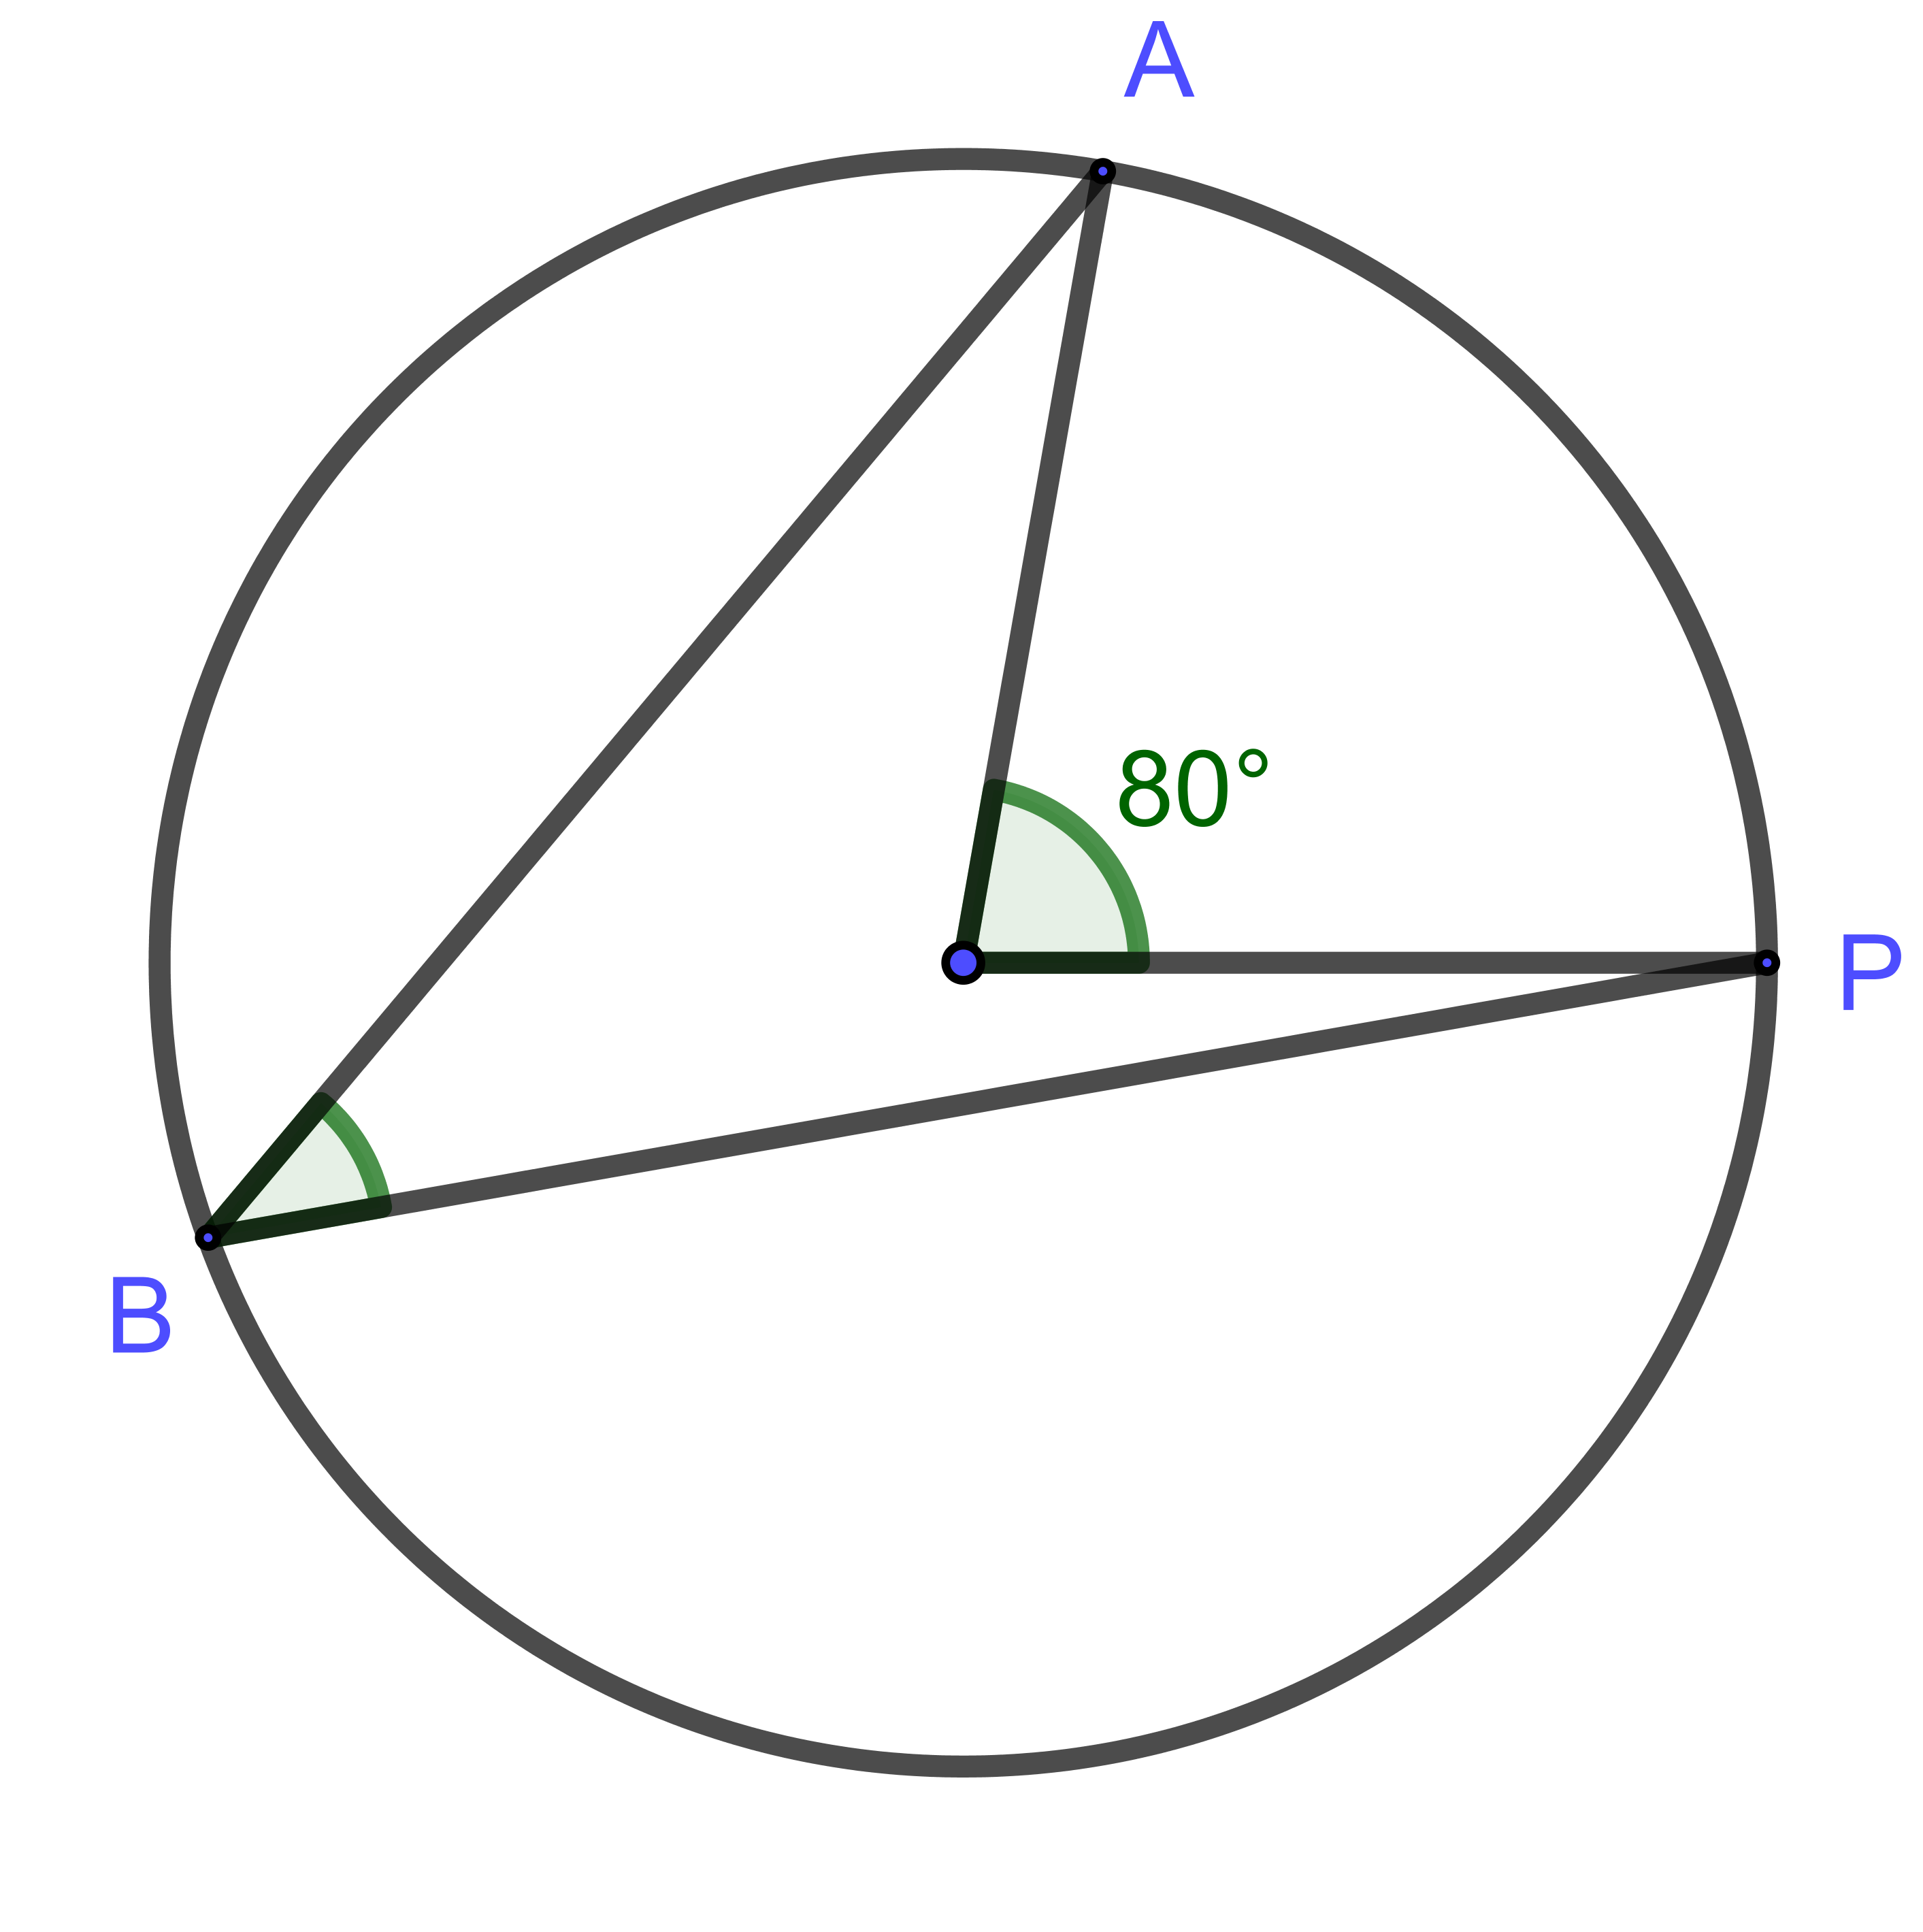
\includegraphics[width=.6\textwidth]{img/3-1_insc_angle_1}
\\\uncover<2>{\red{40\degree}}
\end{minipage}
\begin{minipage}[t]{.49\textwidth}
\ivs
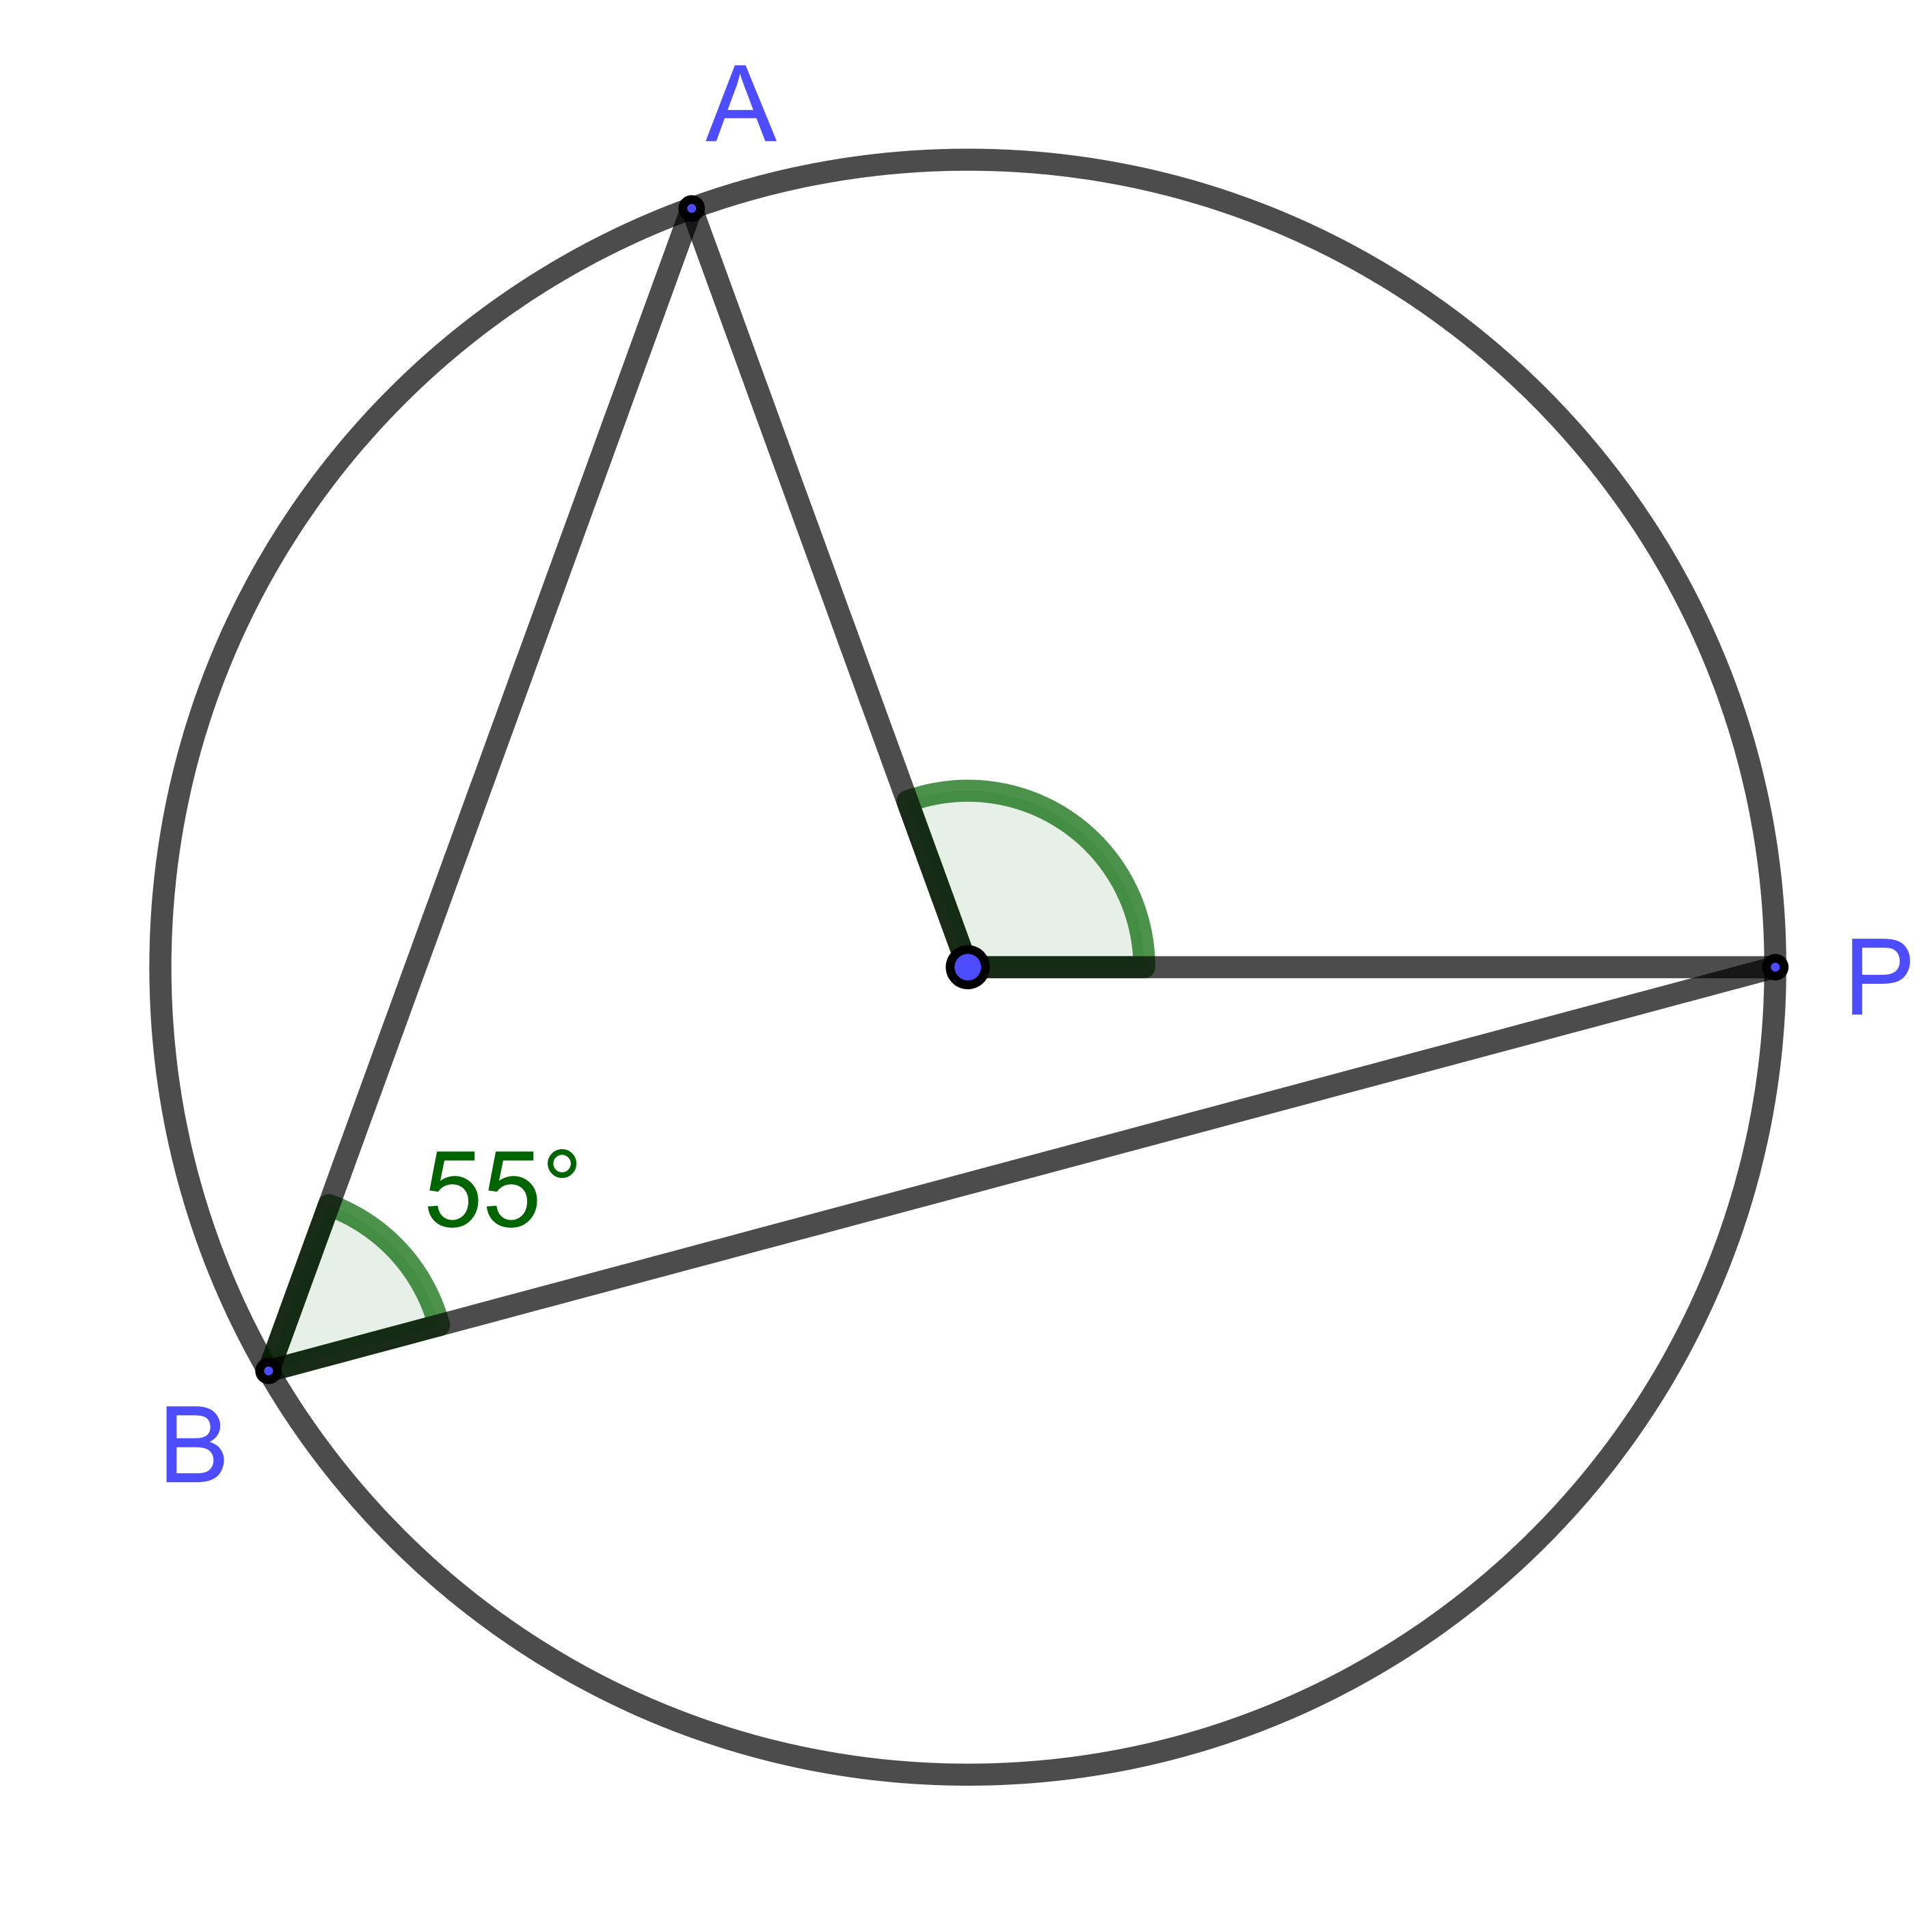
\includegraphics[width=.6\textwidth]{img/3-1_insc_angle_2}
\\\uncover<2>{\red{110\degree}}
\end{minipage}
\par\vspace{20pt}
\begin{minipage}[t]{.49\textwidth}
\ivs
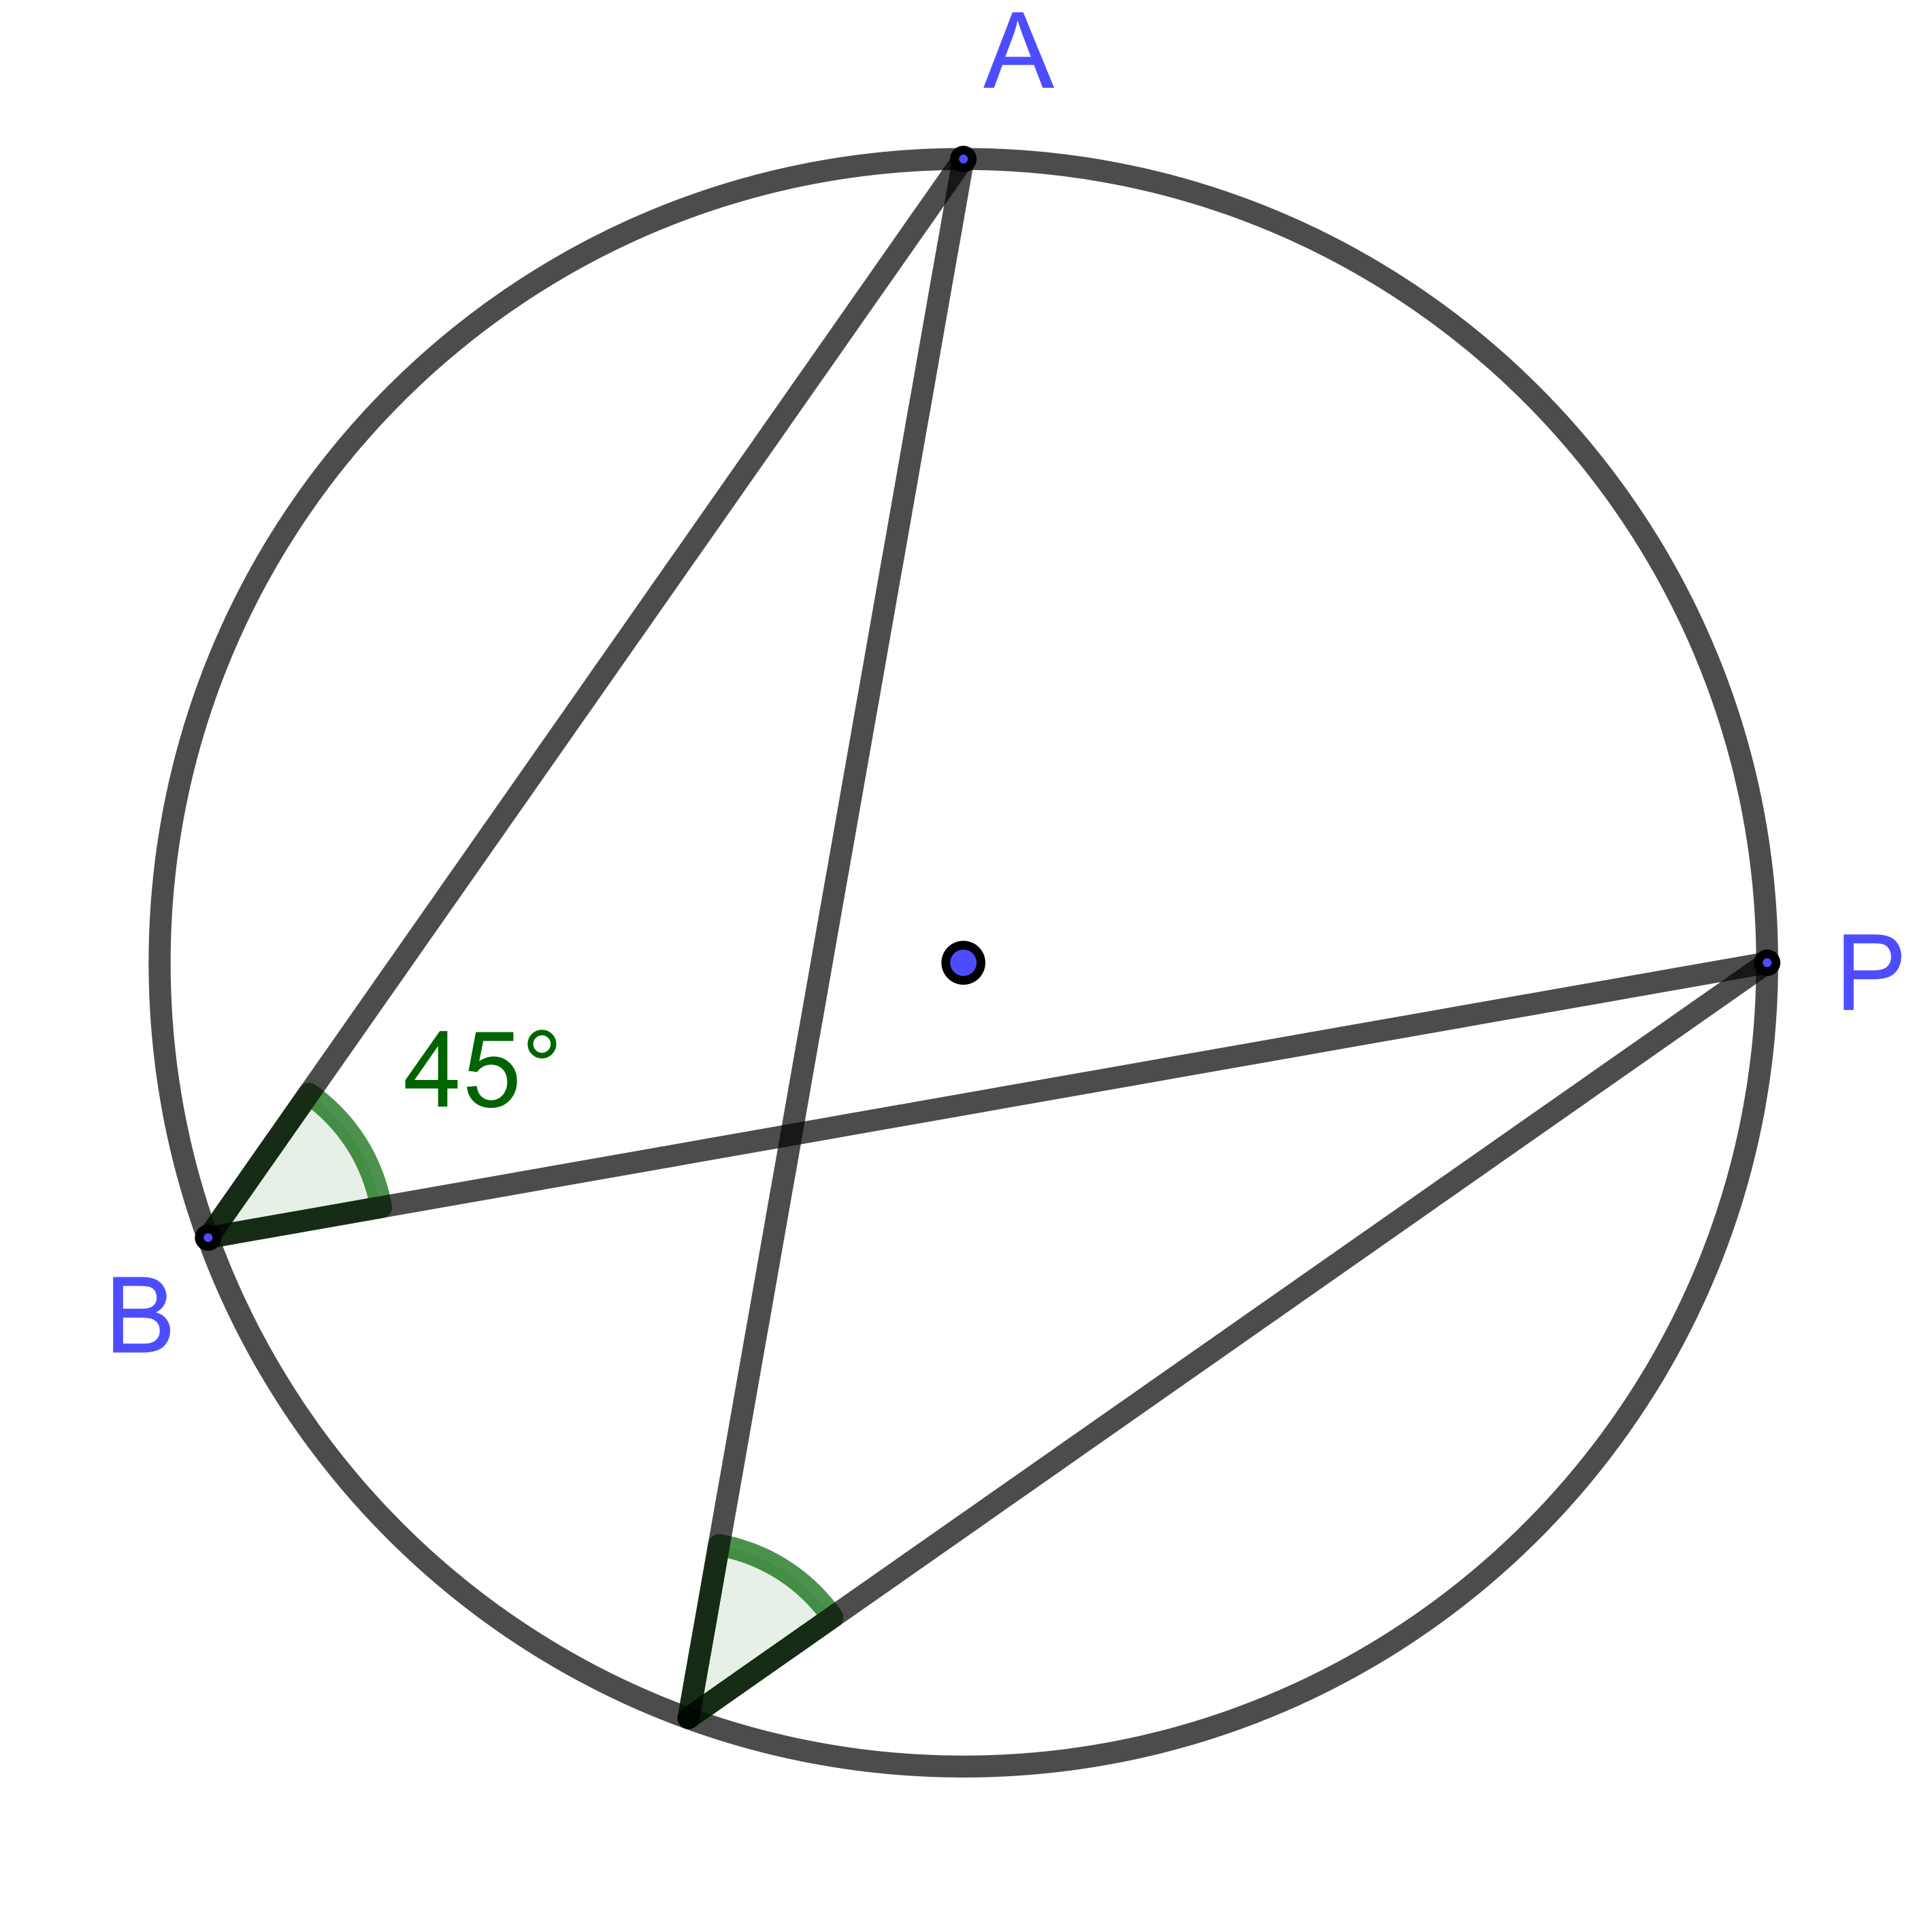
\includegraphics[width=.6\textwidth]{img/3-1_insc_angle_3}
\\\uncover<2>{\red{45\degree}}
\end{minipage}
\begin{minipage}[t]{.49\textwidth}
\ivs
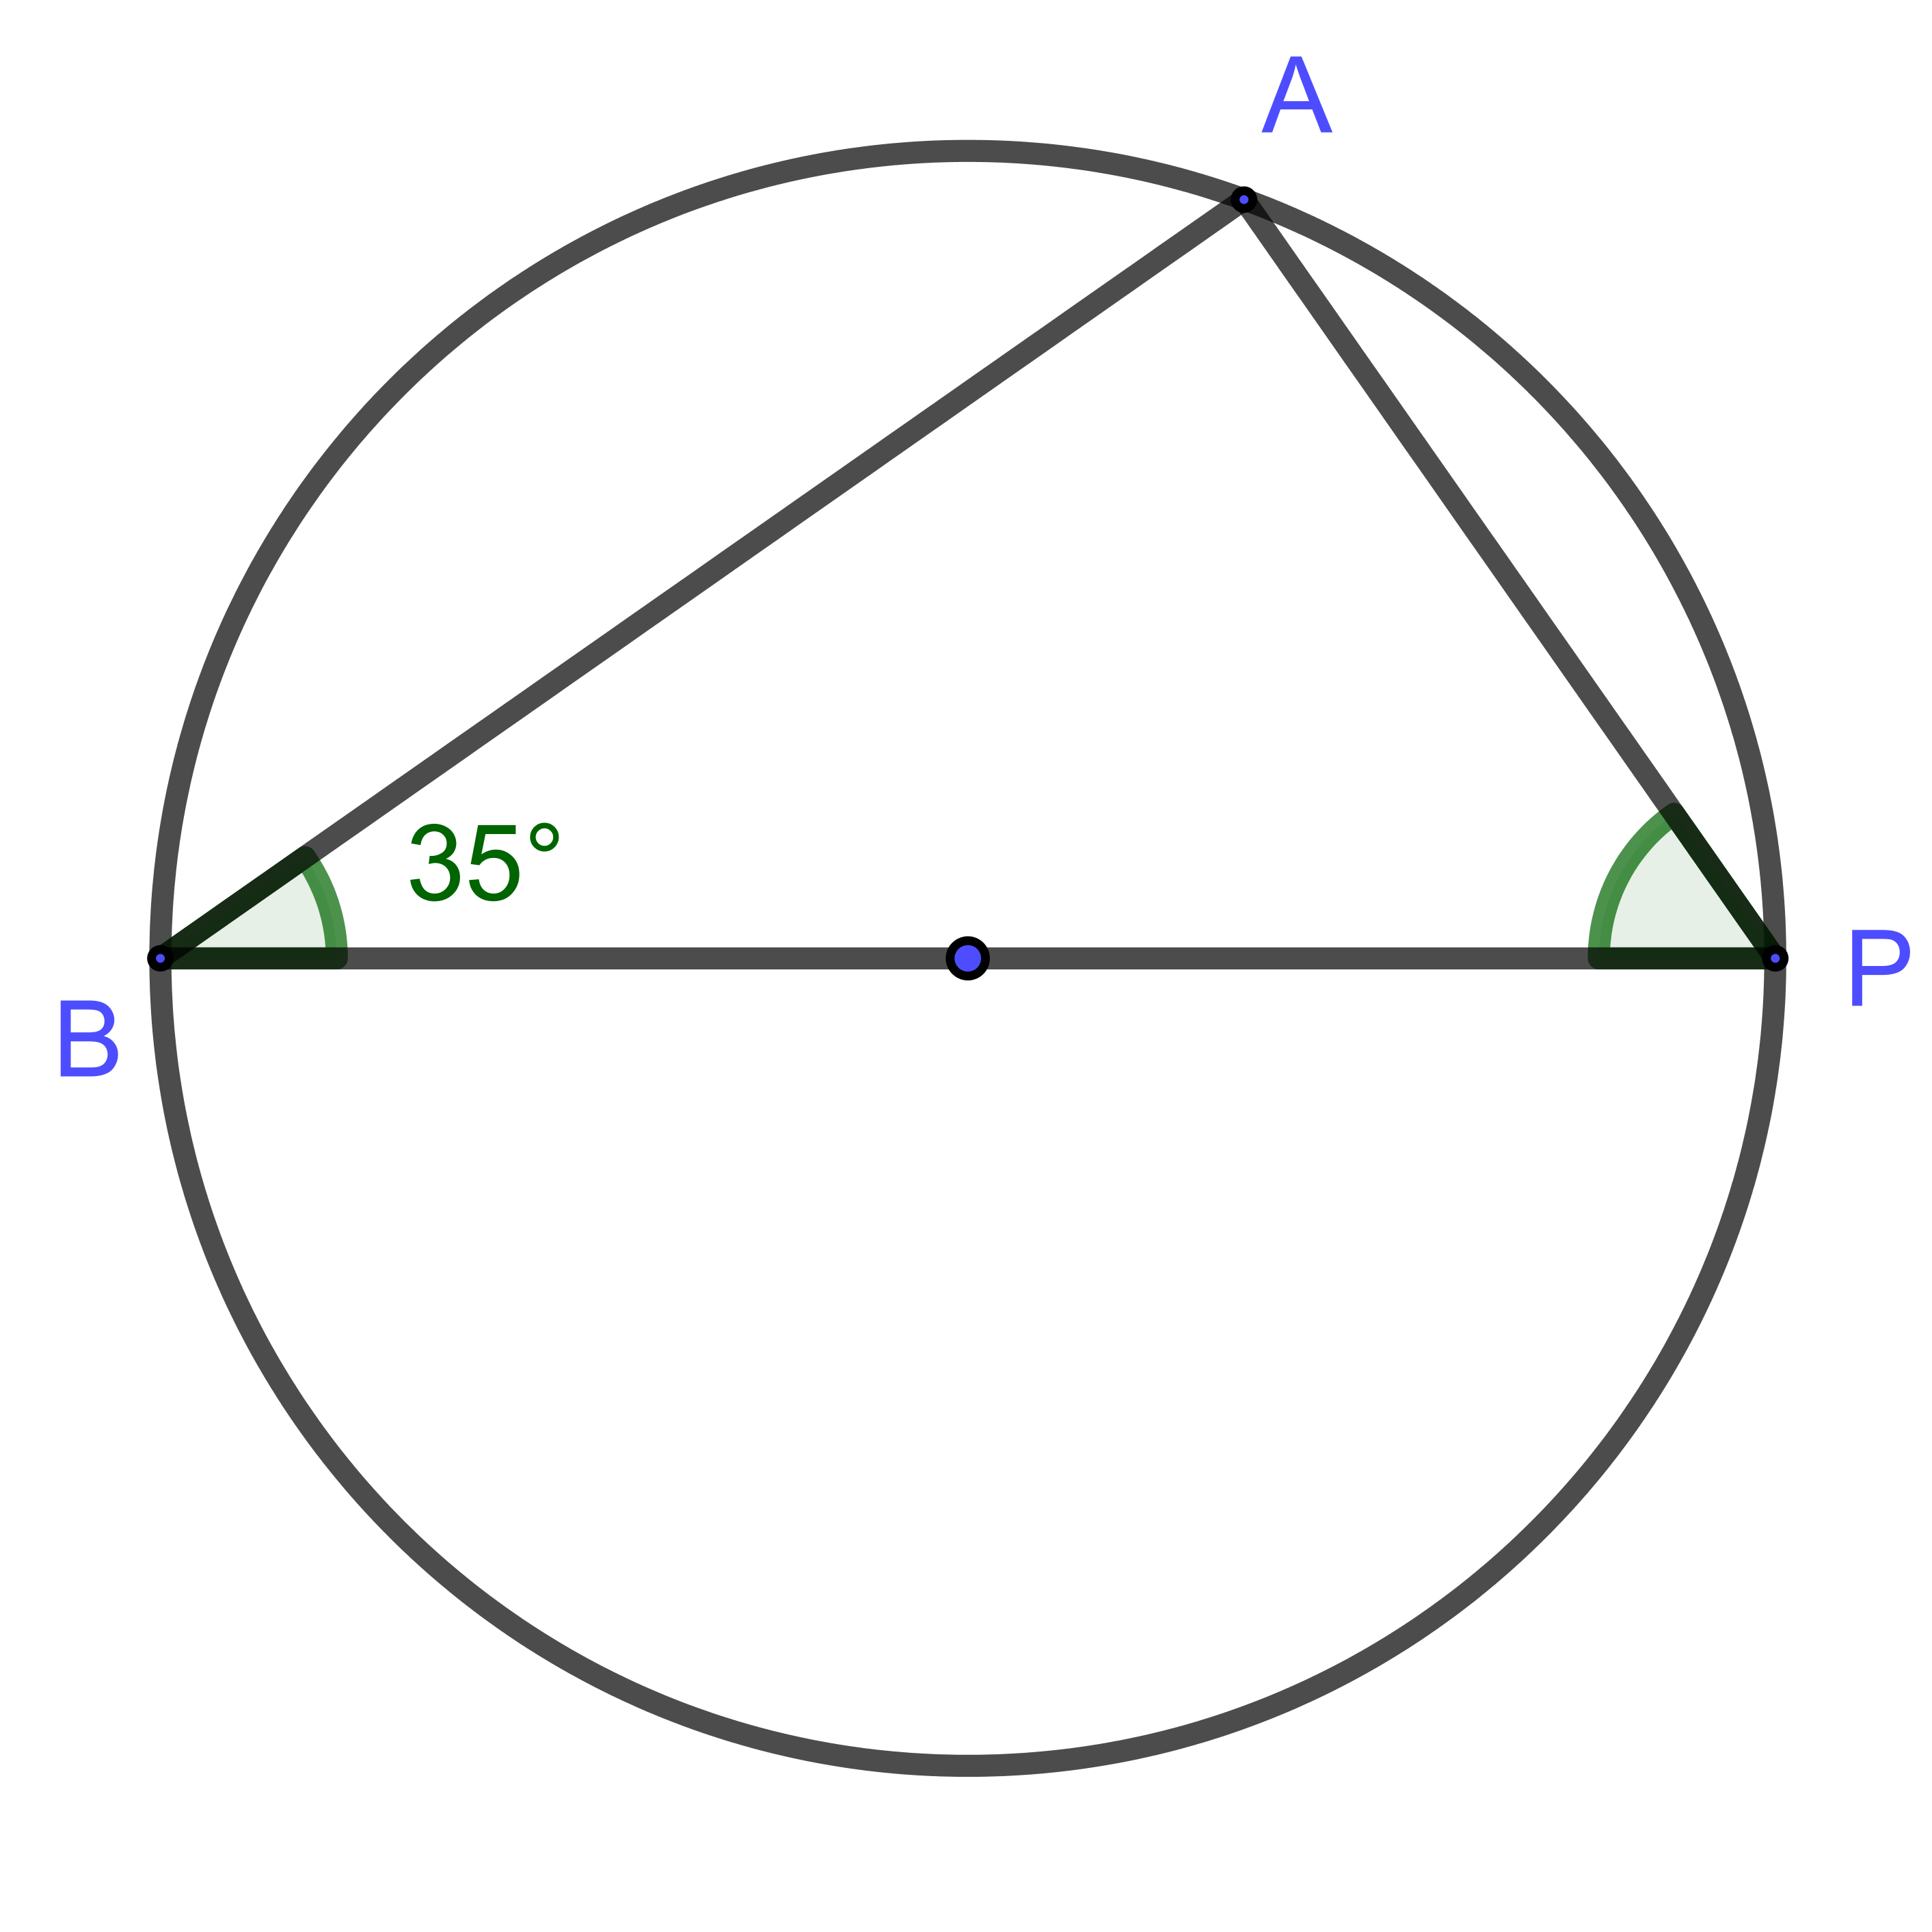
\includegraphics[width=.6\textwidth]{img/3-1_insc_angle_4}
\\\uncover<2>{\red{55\degree}}
\end{minipage}
\end{prob}
\end{frame}

%%%
\subsection{사인 법칙}

%%
\begin{frame}{\subsecname}
\begin{minipage}[c]{.6\textwidth}
%
\begin{theo}{) 사인 법칙}
\[\frac a{\sin A}=\frac b{\sin B}=\frac c{\sin C}=2R\]
\end{theo}
\end{minipage}
\begin{minipage}{.3\textwidth}
\begin{center}
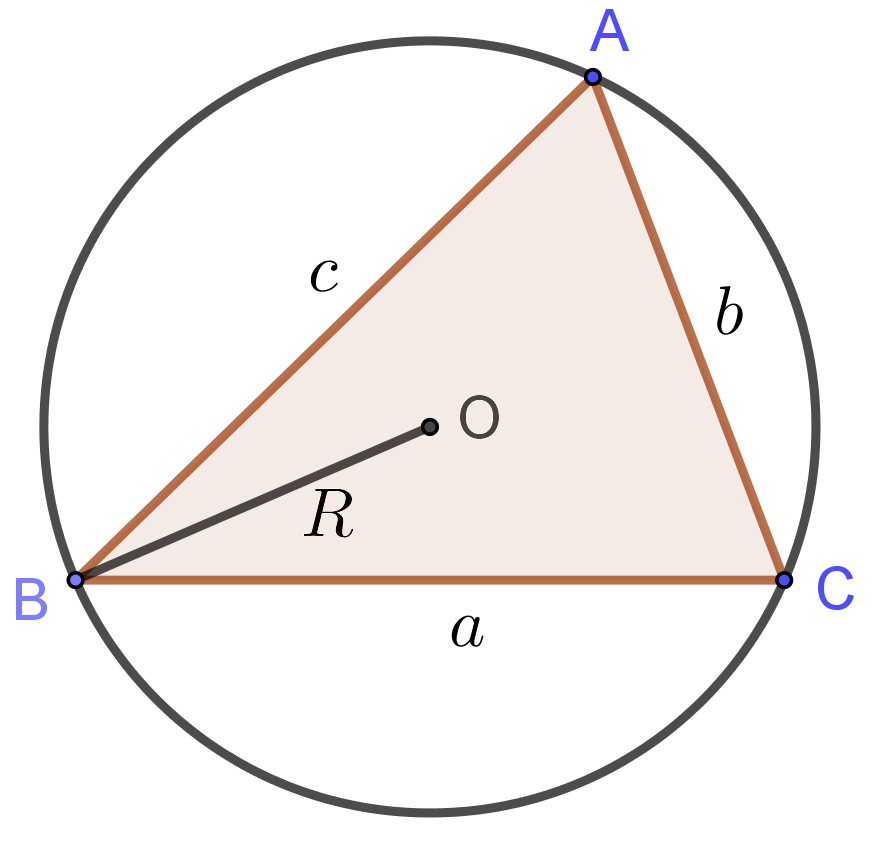
\includegraphics[width=.8\textwidth]{img/3-2_sinlaw_1}
\end{center}
\end{minipage}

\begin{prob}{) 다음 그림에서 \(a\), \(R\), \(\theta\)를 차례로 구하여라.}
\end{prob}
\begin{minipage}{.26\textwidth}\centering
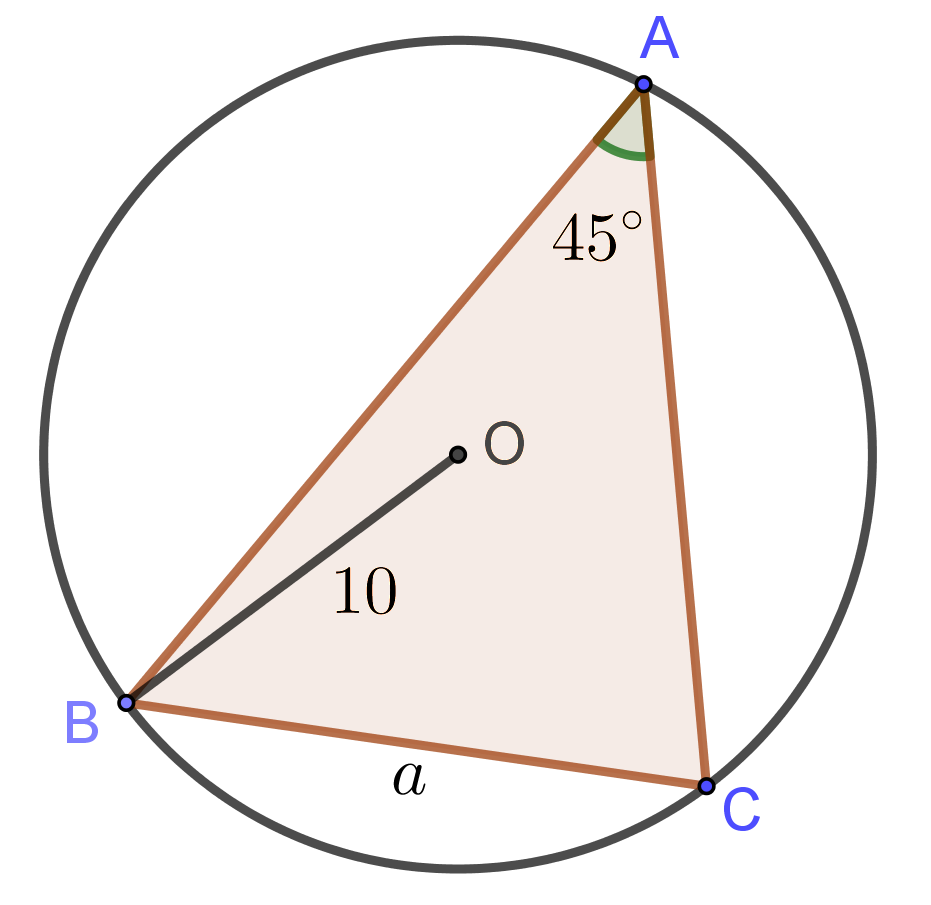
\includegraphics[width=\textwidth]{img/3-2_sinlaw_2-1}
\\\(a=\uncover<2>{\red{10\sqrt2}}\)
\end{minipage}
\qquad
\begin{minipage}{.26\textwidth}\centering
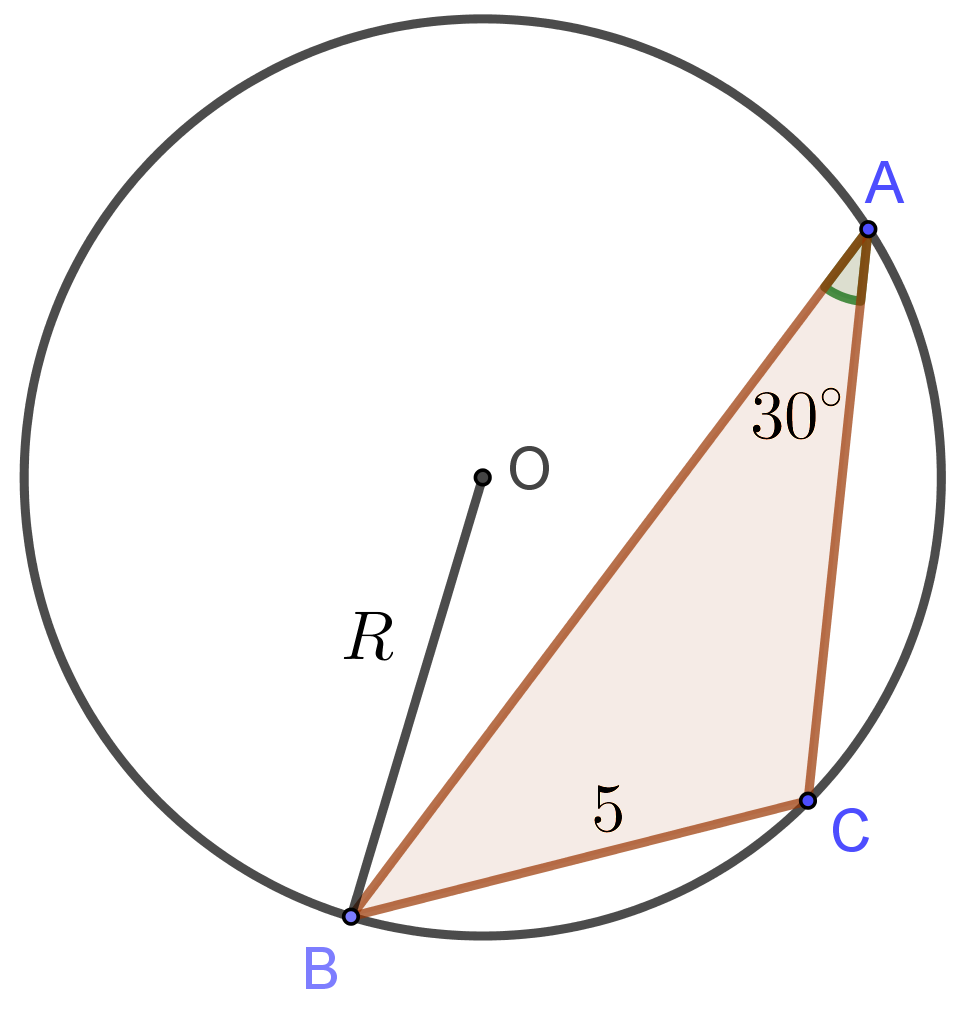
\includegraphics[width=\textwidth]{img/3-2_sinlaw_2-2}
\\\(R=\uncover<2>{\red{5}}\)
\end{minipage}
\qquad
\begin{minipage}{.26\textwidth}\centering
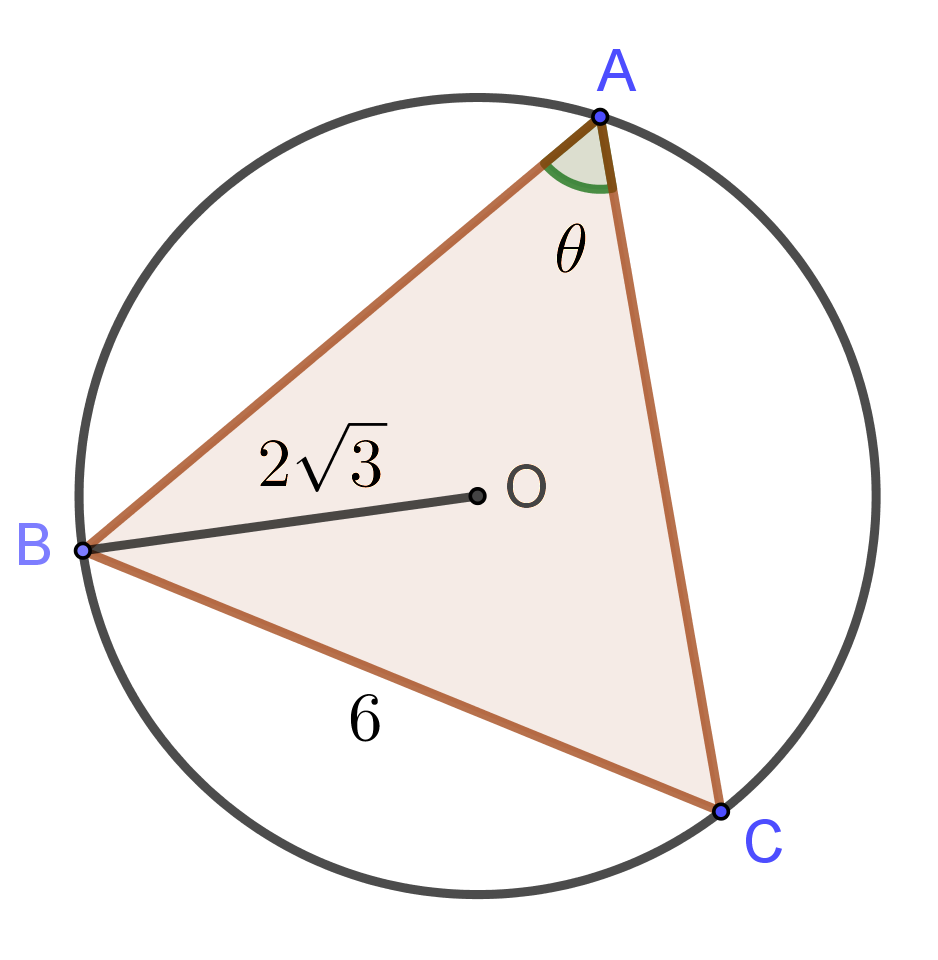
\includegraphics[width=\textwidth]{img/3-2_sinlaw_2-3}
\\\(\theta=\uncover<2>{\red{60\degree}}\)
\end{minipage}
\end{frame}

%%
\begin{frame}{\subsecname}
%
\begin{prob}{) \(c\)의 값을 구하여라.}
\begin{minipage}{.3\textwidth}
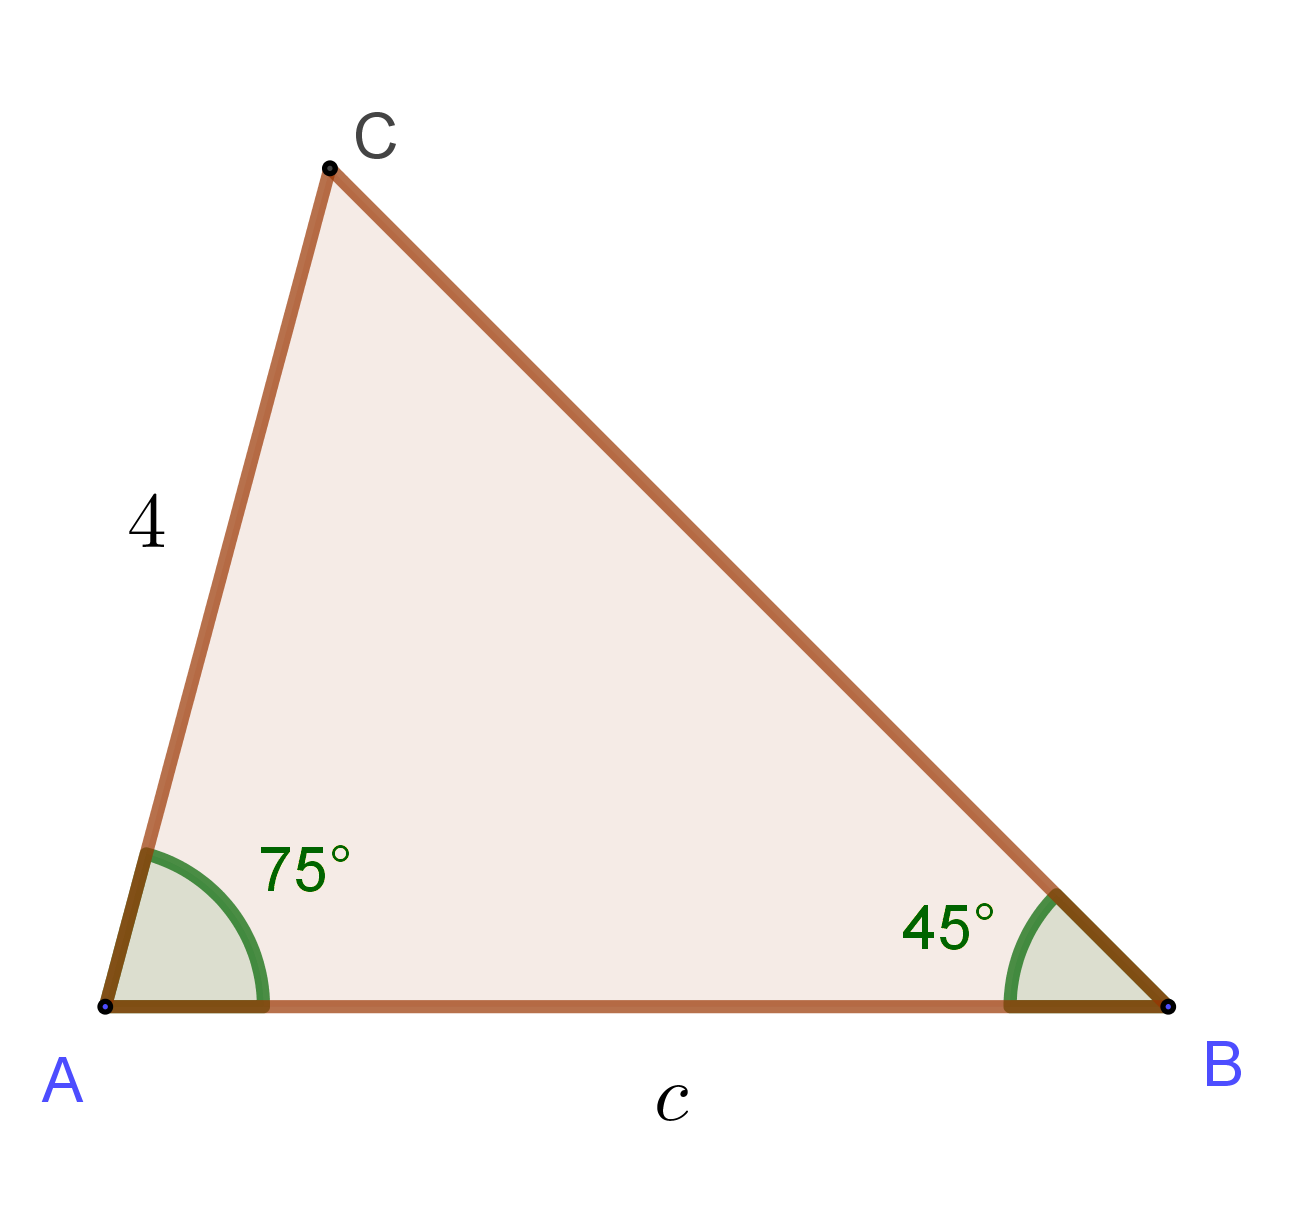
\includegraphics[width=\textwidth]{img/3-2_sinlaw_3}
\end{minipage}
\uncover<2>{\red{\(c=2\sqrt6\)}}
\end{prob}
%
\begin{prob}{) \(a\)의 값을 구하여라.}
\begin{minipage}{.3\textwidth}
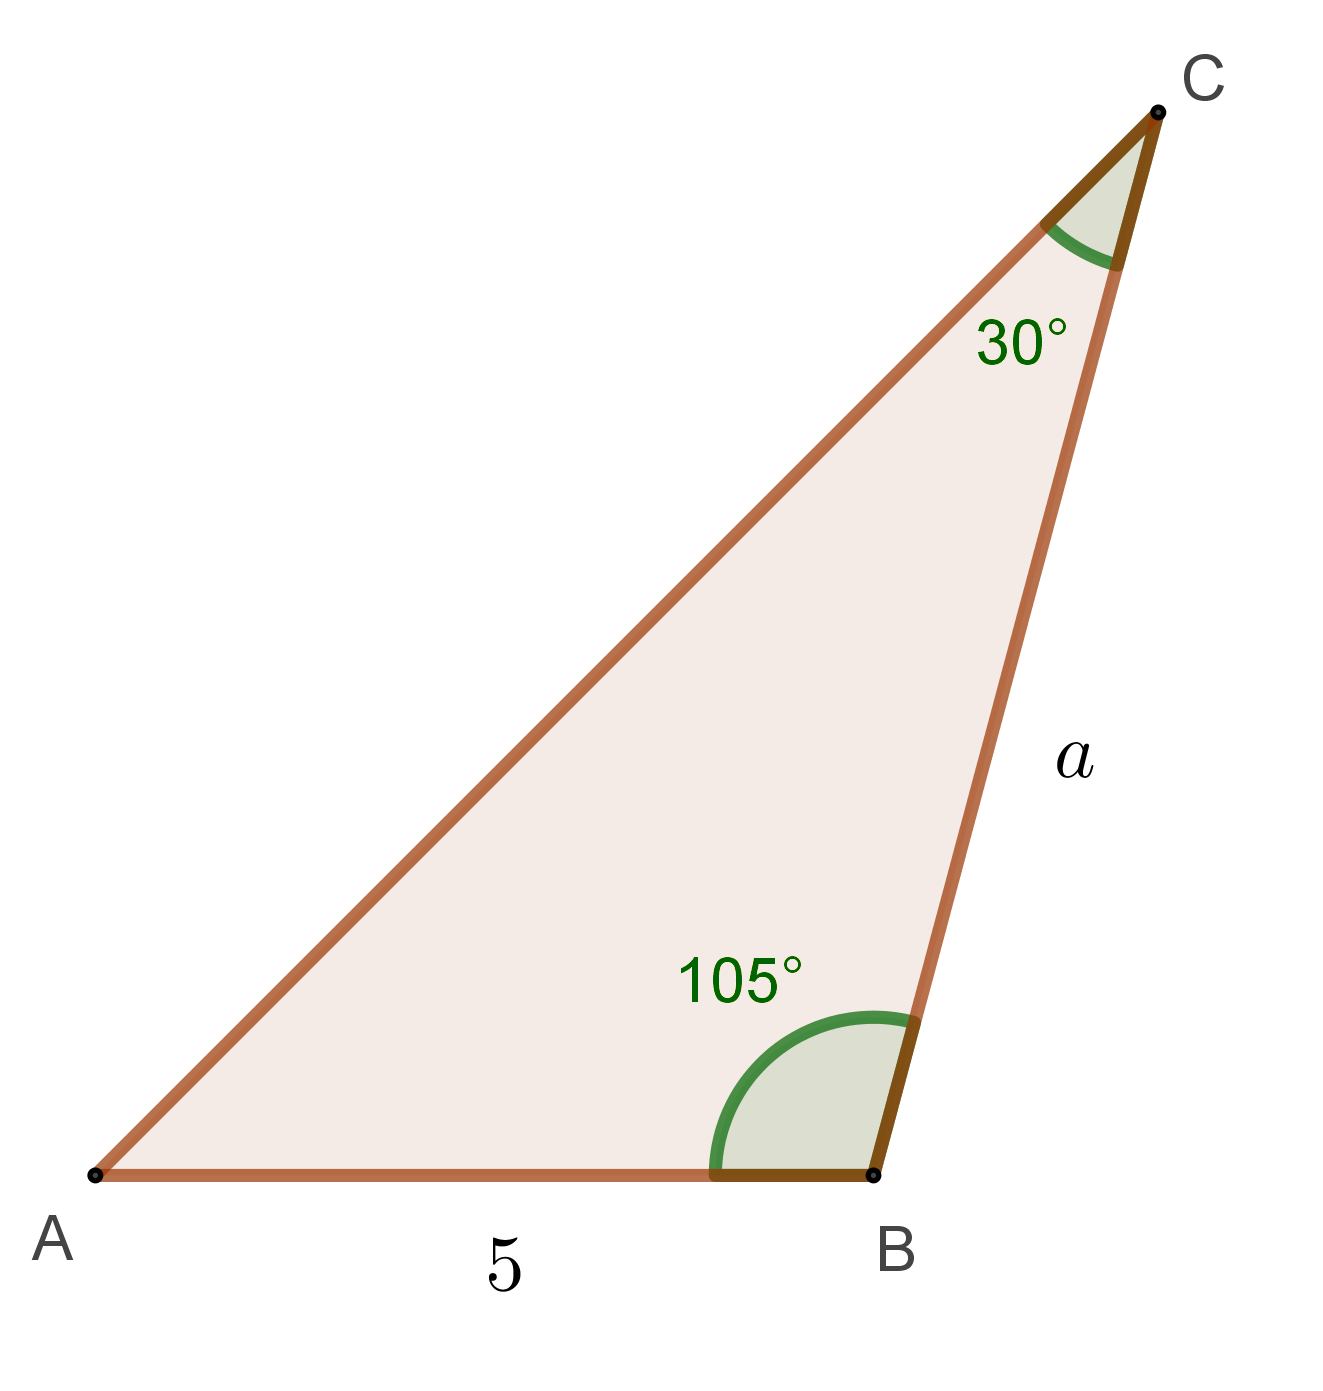
\includegraphics[width=\textwidth]{img/3-2_sinlaw_4}
\end{minipage}
\uncover<2>{\red{\(a=5\sqrt2\)}}
\end{prob}
\end{frame}

%%%
\subsection{피타고라스의 법칙(복습)}

%%
\begin{frame}{\subsecname}
\begin{minipage}[c]{.6\textwidth}
%
\begin{theo}{) 피타고라스의 정리}
\[c^2=a^2+b^2\]
\end{theo}
\end{minipage}
\begin{minipage}{.3\textwidth}
\begin{center}
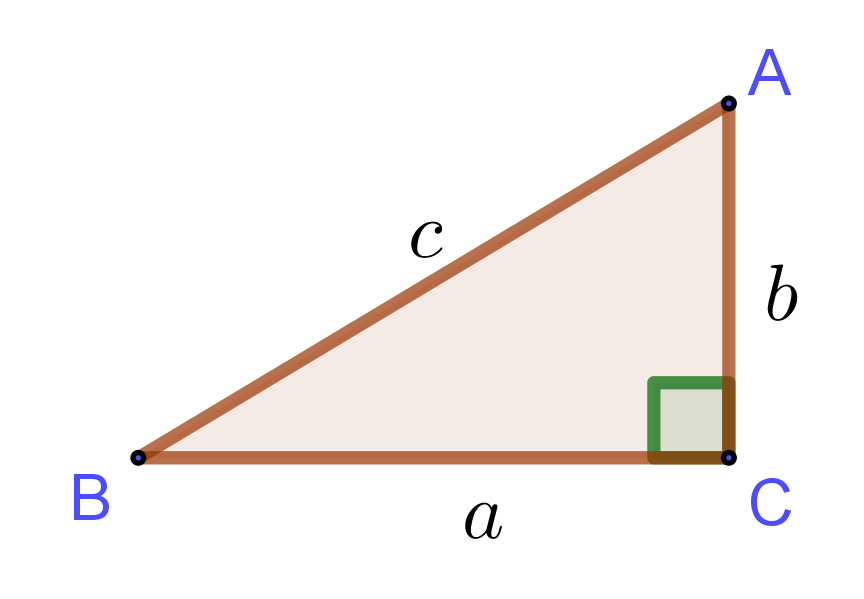
\includegraphics[width=.8\textwidth]{img/3-3_coslaw_1-1}
\end{center}
\end{minipage}
\pause
%
\begin{prob}{) \(c\)를 차례로 구하여라.}
\end{prob}
\begin{minipage}{.26\textwidth}\centering
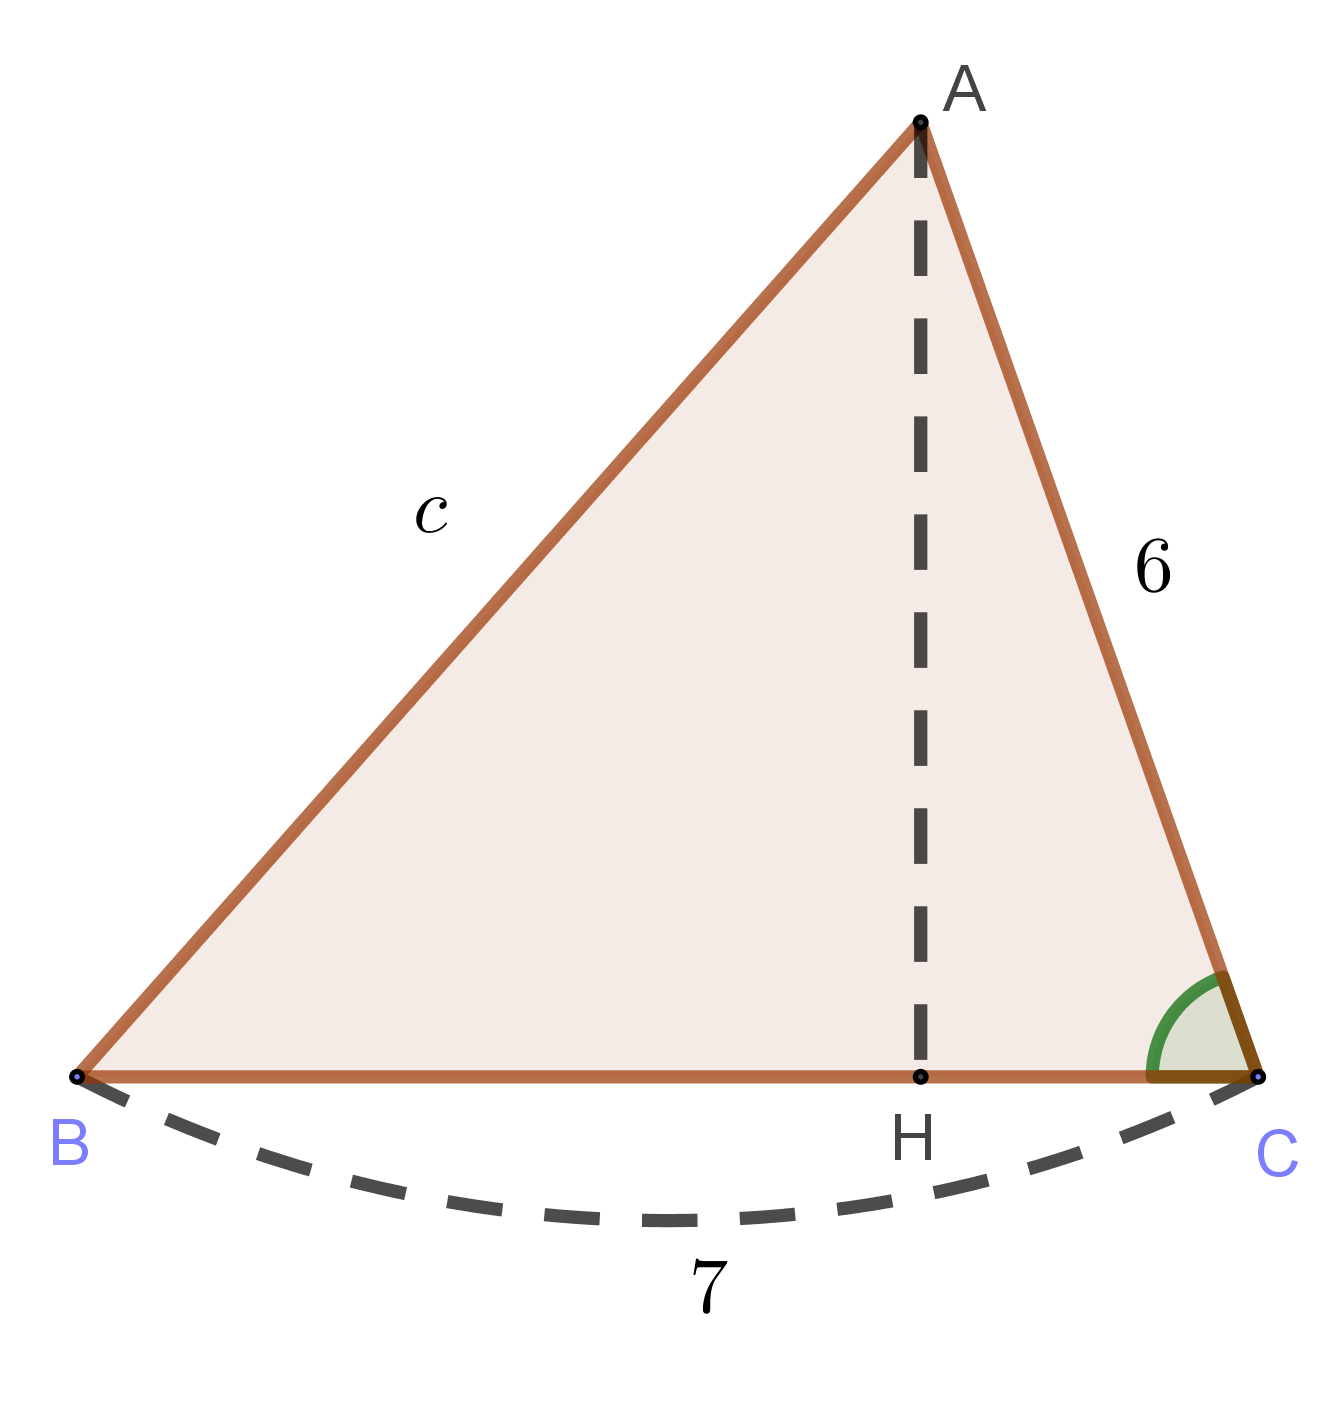
\includegraphics[width=\textwidth]{img/3-3_coslaw_2-1}
\end{minipage}
\begin{minipage}{.15\textwidth}\centering
\(\cos C=\frac13\)\\[20pt]
\(c=\uncover<3->{\red{\sqrt{57}}}\)
\end{minipage}
\qquad\qquad\quad
\begin{minipage}{.26\textwidth}\centering
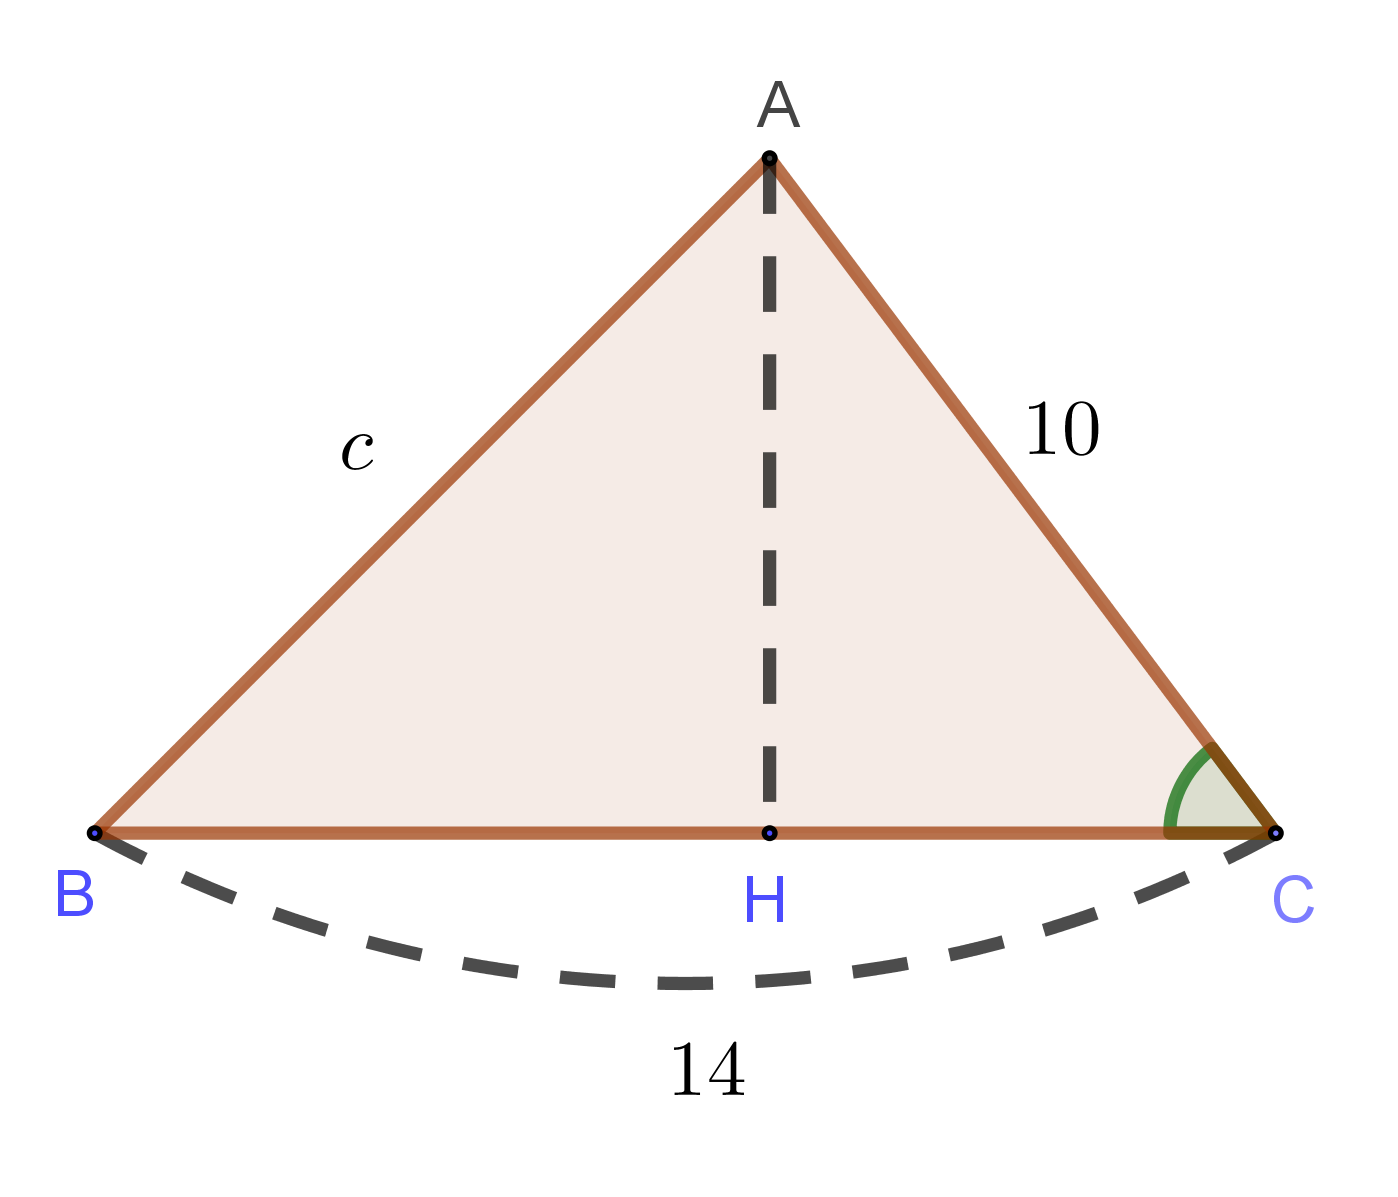
\includegraphics[width=\textwidth]{img/3-3_coslaw_2-2}
\end{minipage}
\begin{minipage}{.15\textwidth}\centering
\(\cos C=\frac35\)\\[20pt]
\(c=\uncover<3->{\red{8\sqrt2}}\)
\end{minipage}

\begin{minipage}{.26\textwidth}\centering
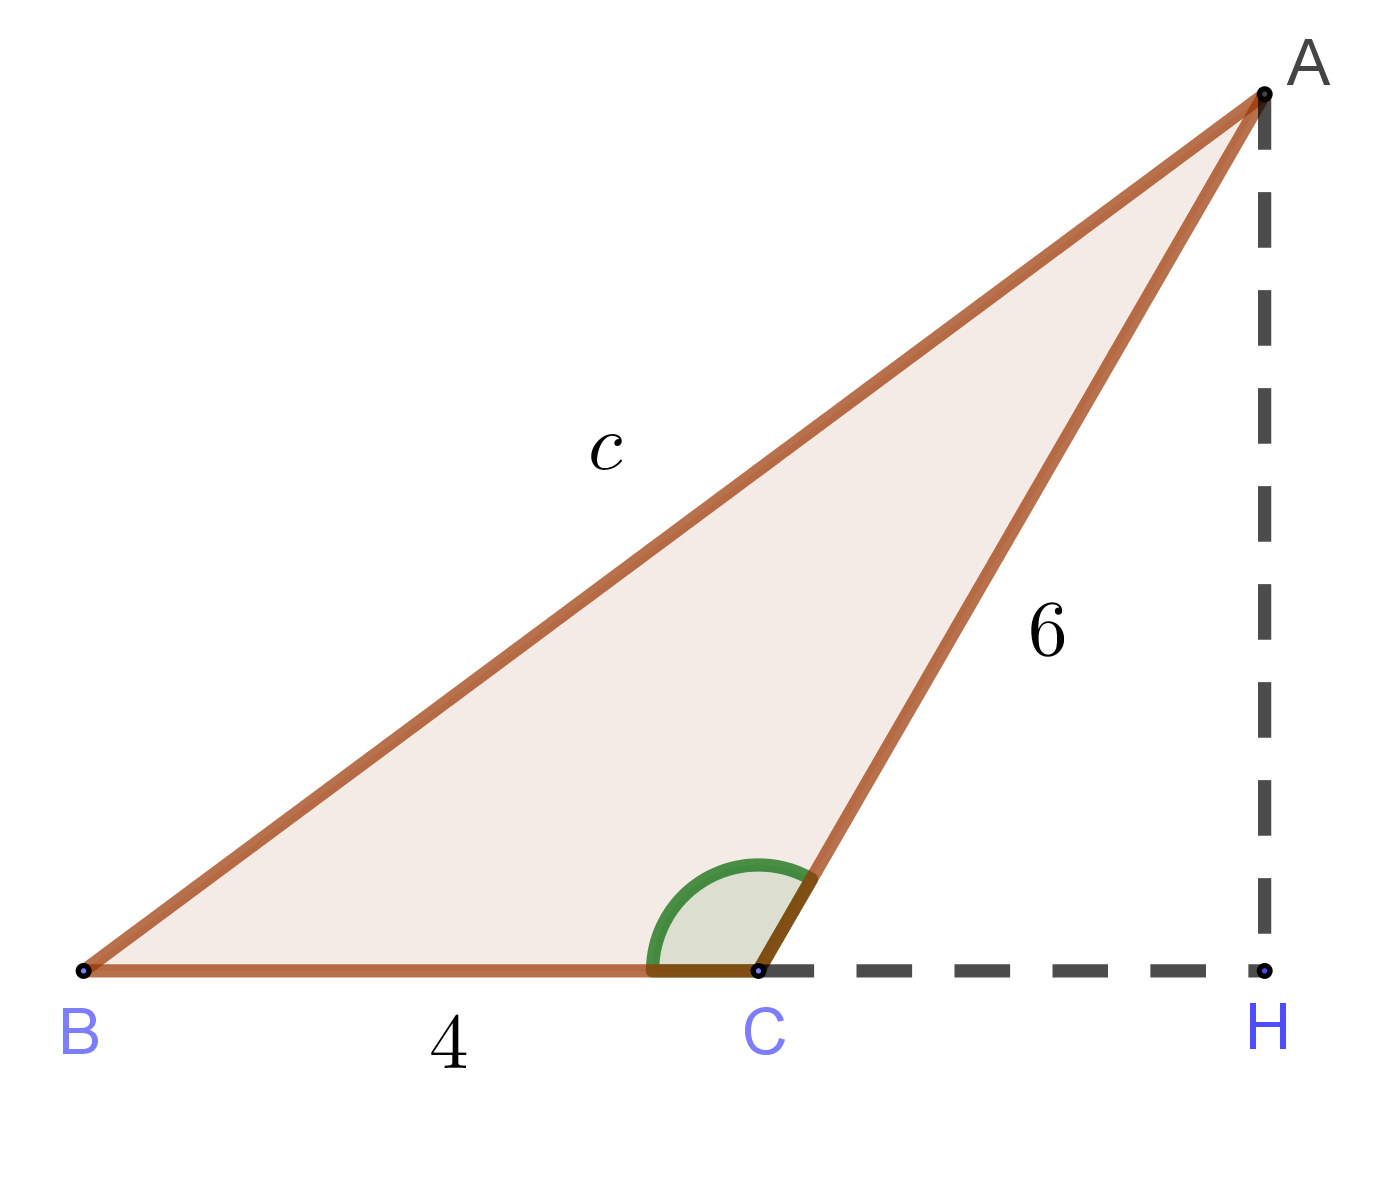
\includegraphics[width=\textwidth]{img/3-3_coslaw_2-3}
\end{minipage}
\begin{minipage}{.15\textwidth}\centering
\(\cos C=-\frac12\)\\[20pt]
\(c=\uncover<3->{\red{2\sqrt{19}}}\)
\end{minipage}
\qquad\qquad\quad
\begin{minipage}{.26\textwidth}\centering
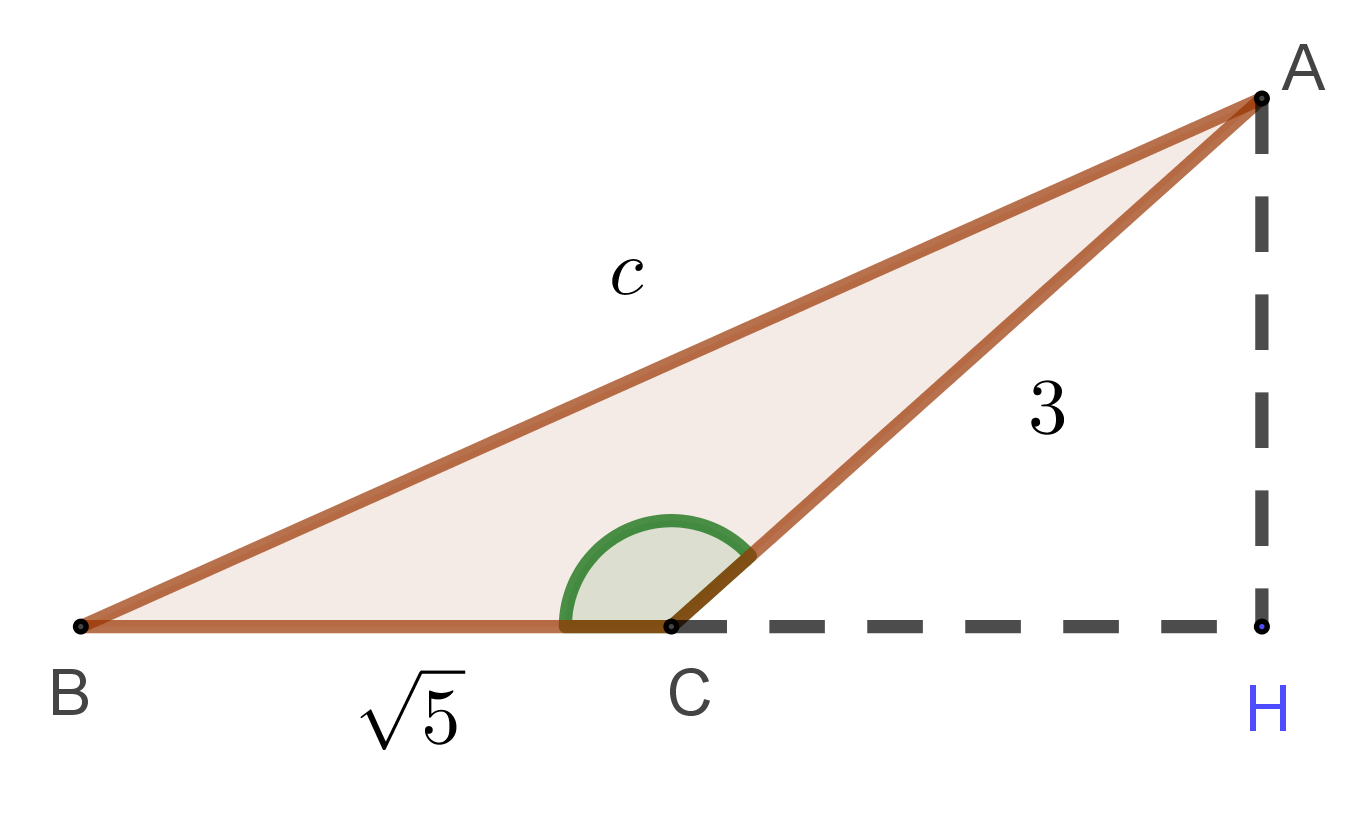
\includegraphics[width=\textwidth]{img/3-3_coslaw_2-4}
\end{minipage}
\begin{minipage}{.15\textwidth}\centering
\(\cos C=-\frac{\sqrt5}3\)\\[20pt]
\(c=\uncover<3->{\red{2\sqrt6}}\)
\end{minipage}
\end{frame}

%%%
\subsection{코사인 법칙}

%%
\begin{frame}{\subsecname}
\begin{minipage}[c]{.6\textwidth}
%
\begin{theo}{) 코사인 법칙}
\[c^2=a^2+b^2-2ab\cos C\]
\end{theo}
\end{minipage}
\begin{minipage}{.3\textwidth}
\begin{center}
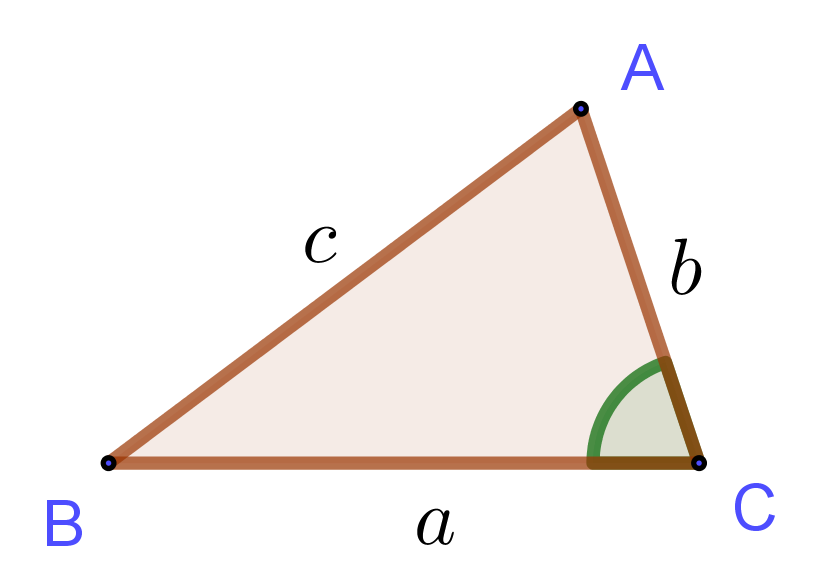
\includegraphics[width=.8\textwidth]{img/3-3_coslaw_1-2}
\end{center}
\end{minipage}

\pause
%
\begin{prob}{) \(c\)를 차례로 구하여라.}
\end{prob}
\begin{minipage}{.26\textwidth}\centering
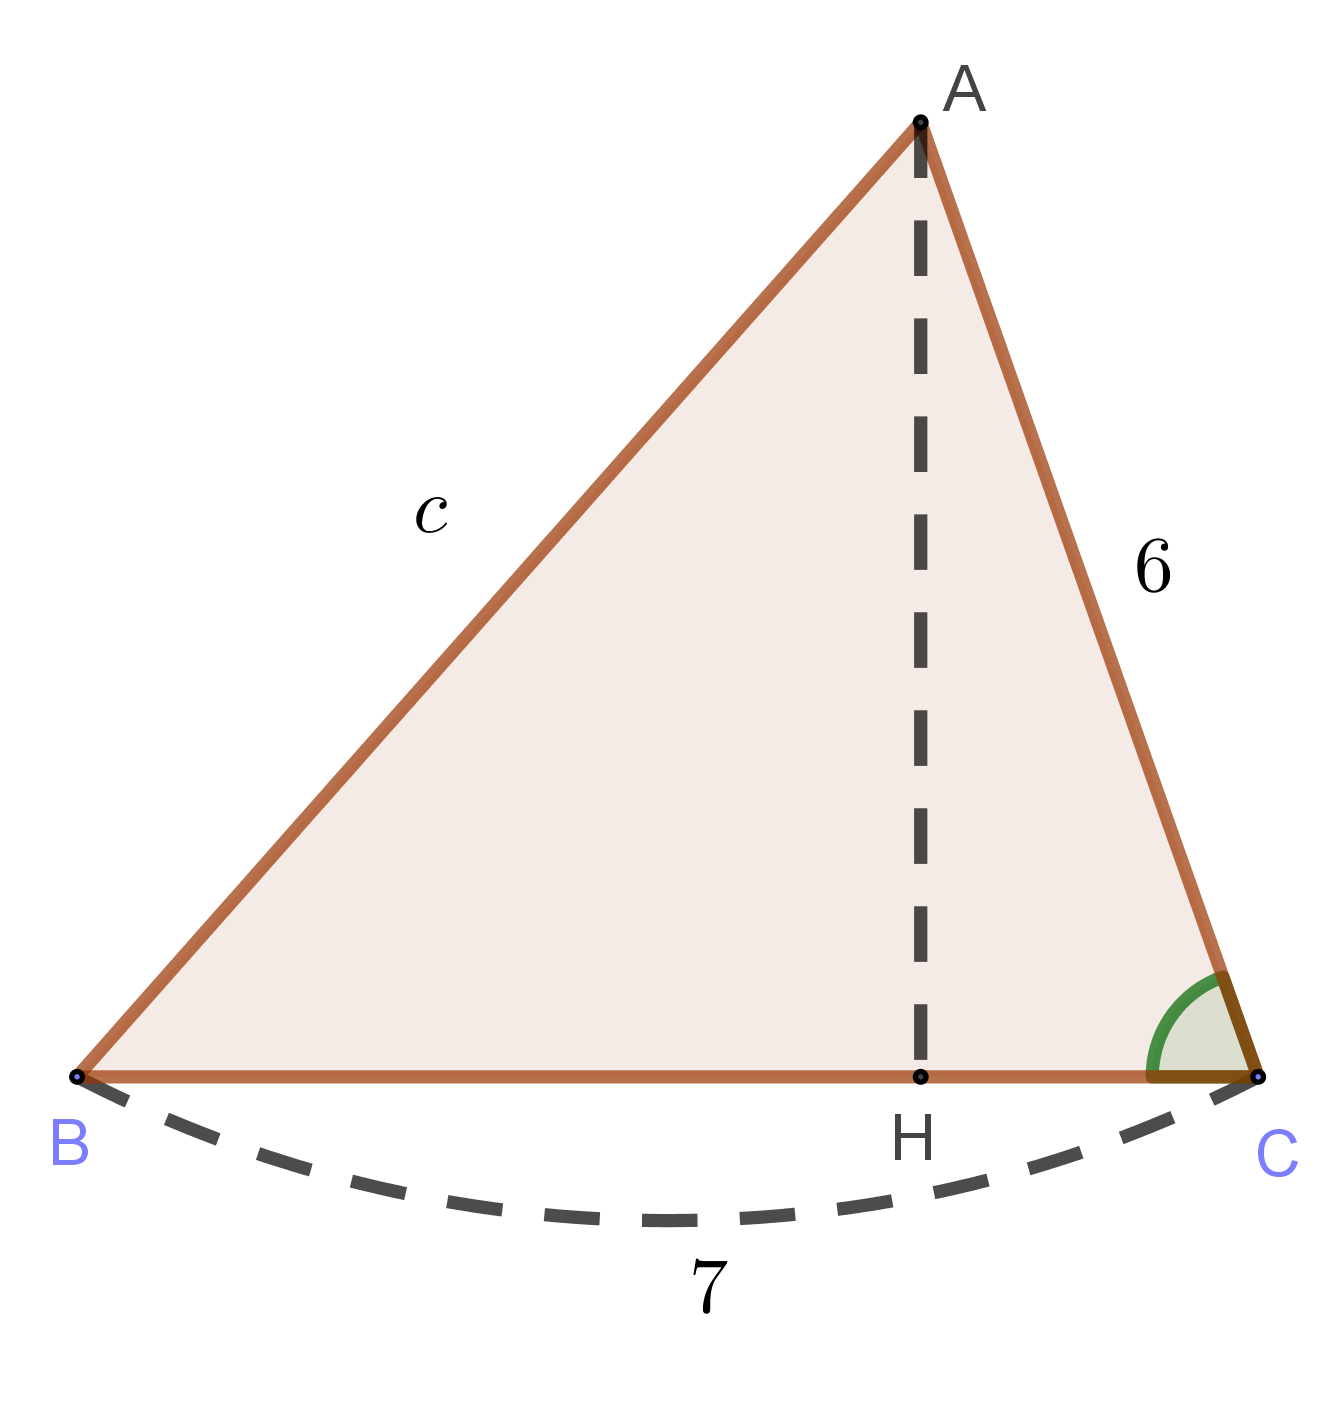
\includegraphics[width=\textwidth]{img/3-3_coslaw_2-1}
\end{minipage}
\begin{minipage}{.15\textwidth}\centering
\(\cos C=\frac13\)\\[20pt]
\(c=\uncover<3->{\red{\sqrt{57}}}\)
\end{minipage}
\qquad\qquad\quad
\begin{minipage}{.26\textwidth}\centering
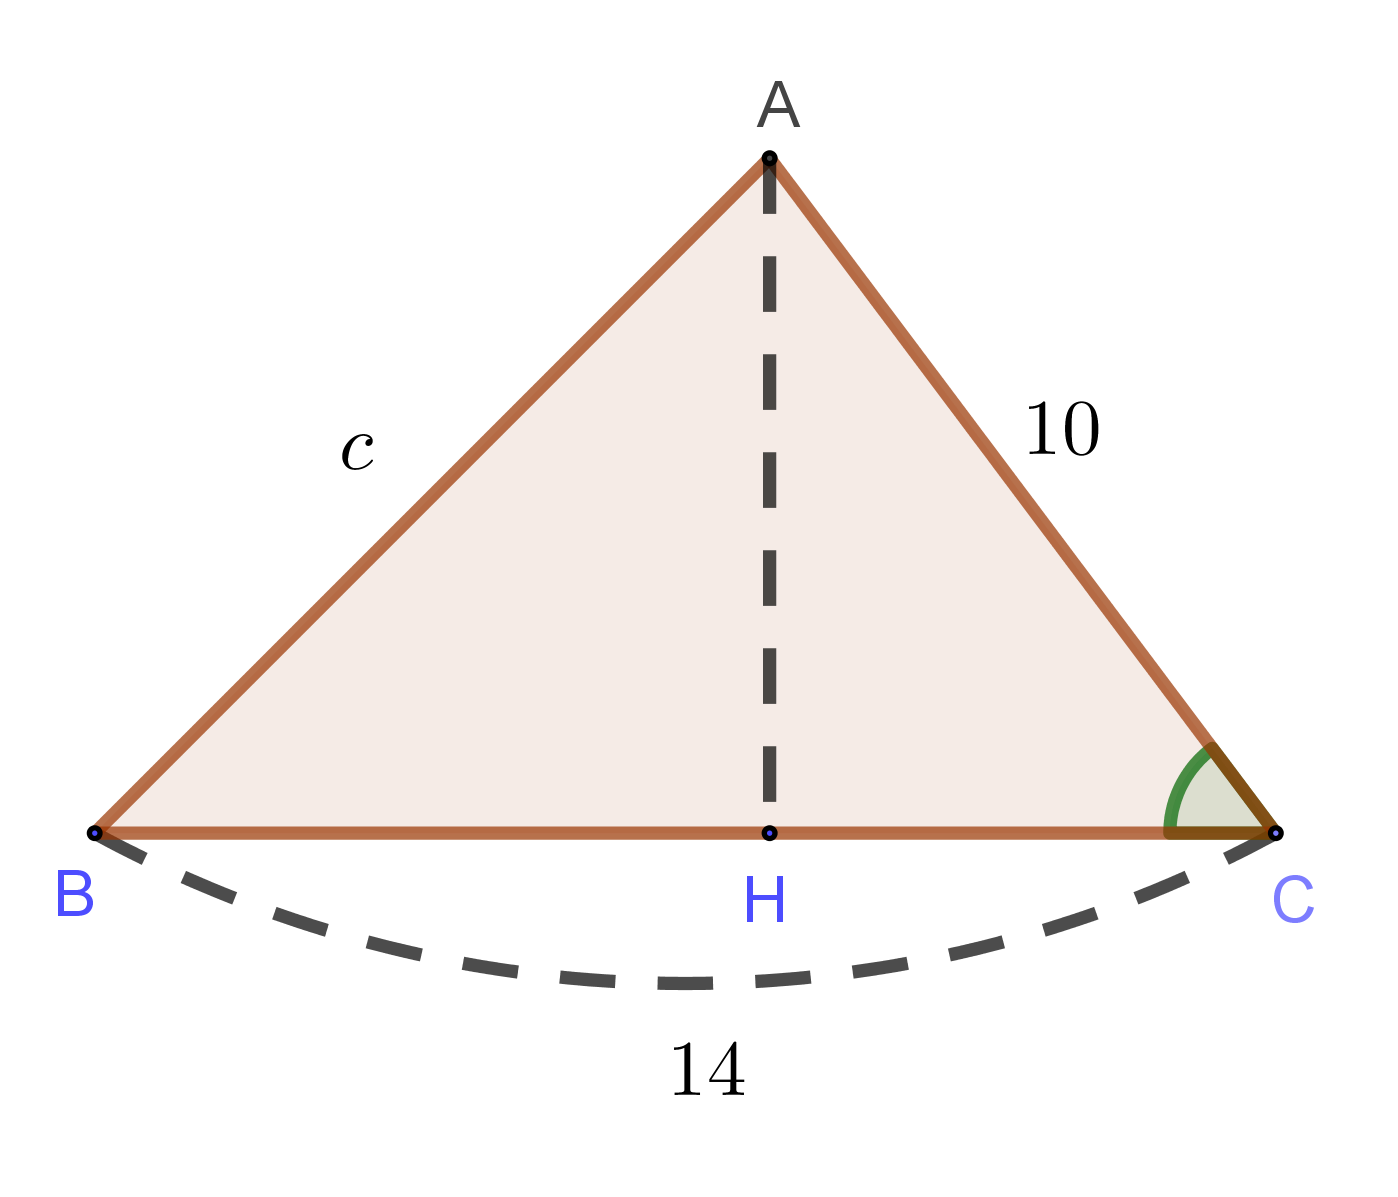
\includegraphics[width=\textwidth]{img/3-3_coslaw_2-2}
\end{minipage}
\begin{minipage}{.15\textwidth}\centering
\(\cos C=\frac35\)\\[20pt]
\(c=\uncover<3->{\red{8\sqrt2}}\)
\end{minipage}

\begin{minipage}{.26\textwidth}\centering
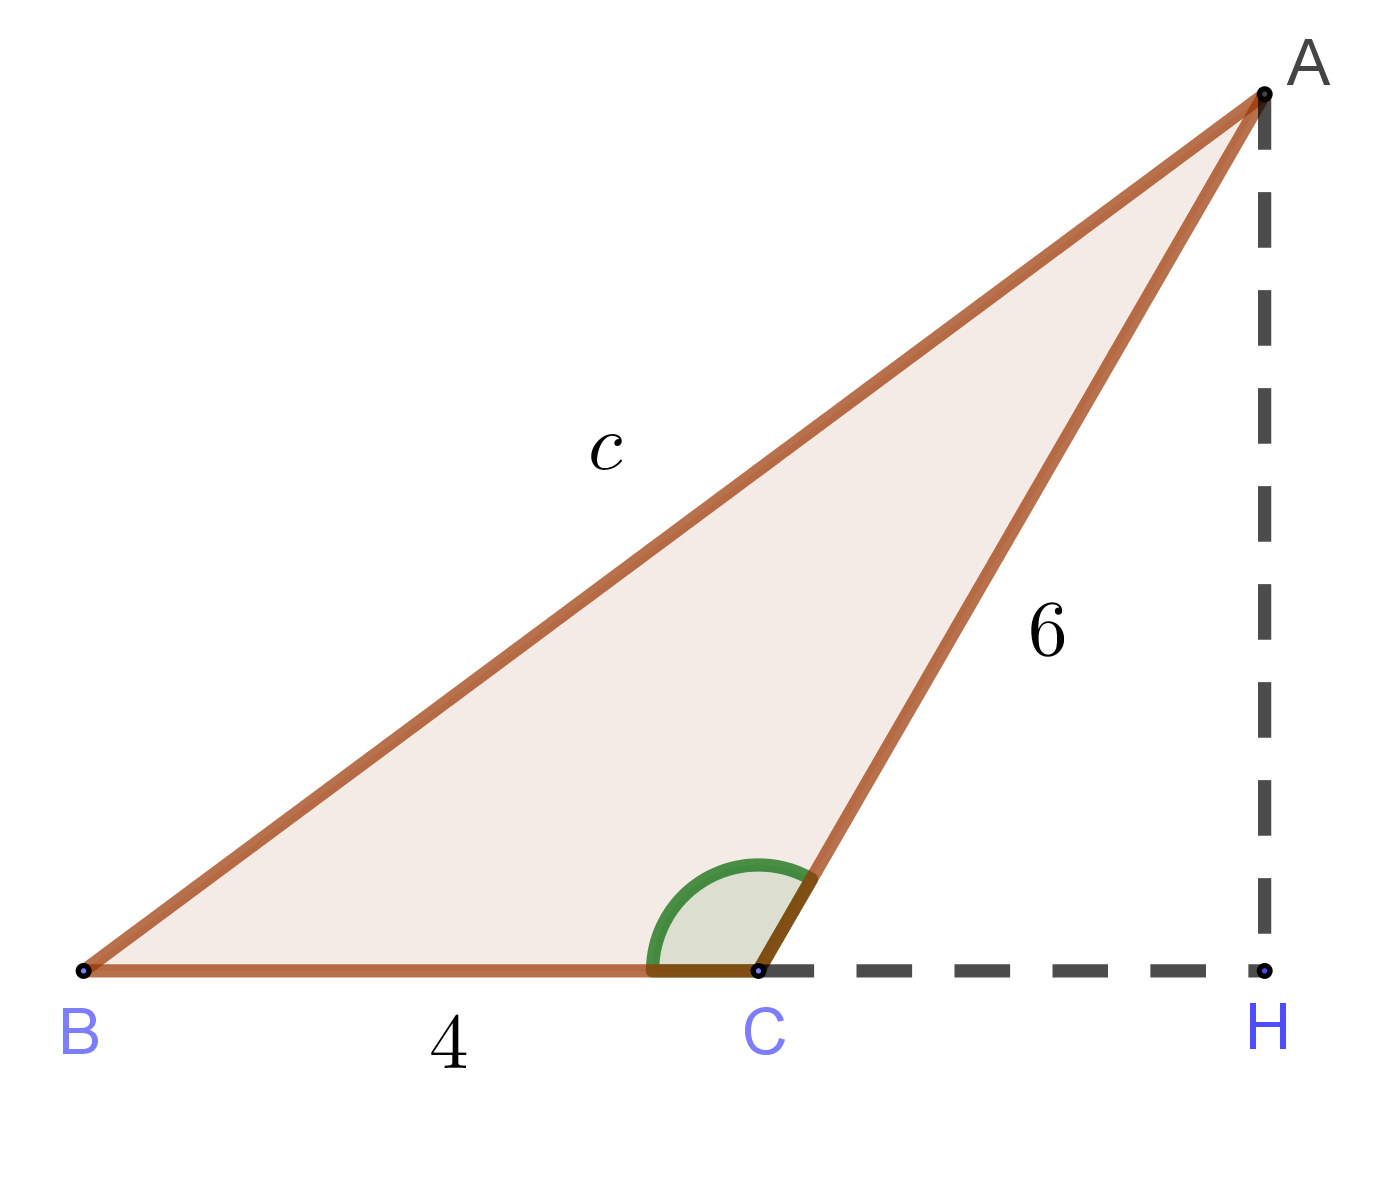
\includegraphics[width=\textwidth]{img/3-3_coslaw_2-3}
\end{minipage}
\begin{minipage}{.15\textwidth}\centering
\(\cos C=-\frac12\)\\[20pt]
\(c=\uncover<3->{\red{2\sqrt{19}}}\)
\end{minipage}
\qquad\qquad\quad
\begin{minipage}{.26\textwidth}\centering
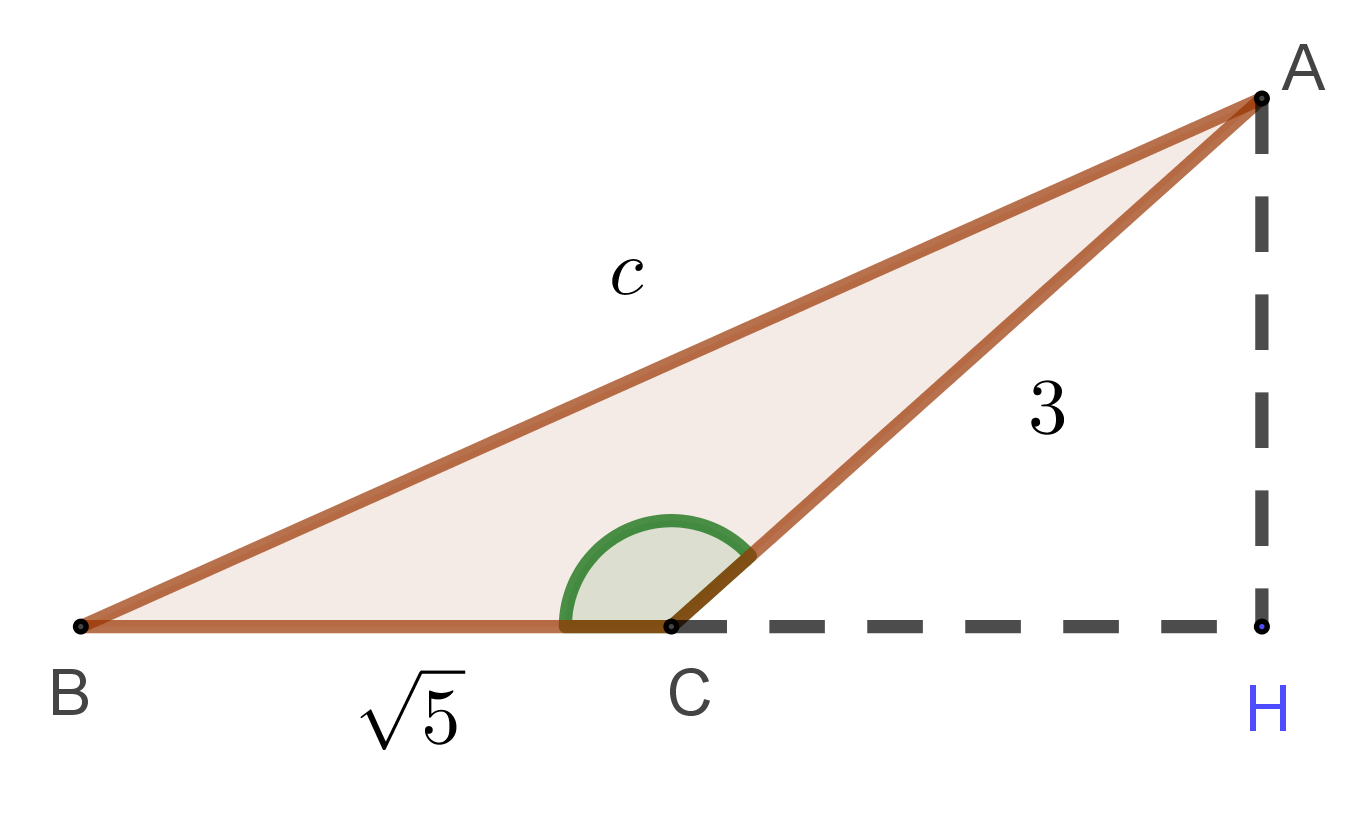
\includegraphics[width=\textwidth]{img/3-3_coslaw_2-4}
\end{minipage}
\begin{minipage}{.15\textwidth}\centering
\(\cos C=-\frac{\sqrt5}3\)\\[20pt]
\(c=\uncover<3->{\red{2\sqrt6}}\)
\end{minipage}
\end{frame}



\end{document}